% !TEX root = ./paper.tex
% !TEX engine = latexmk -pdf
% !TEX buildOnSave = true
\documentclass[sigconf]{acmart}

\usepackage[english]{babel}
\usepackage{enumitem}
\usepackage{hyperref}
\usepackage{verbatim}
\usepackage{tikz}
\usepackage{pifont}% http://ctan.org/pkg/pifont
\newcommand{\cmark}{\ding{51}}%
\newcommand{\xmark}{\ding{55}}%
\usepackage{listings}

\usepackage{bytefield}
\usepackage{paralist}
\usepackage[htt]{hyphenat}
\usepackage{xspace}
\usetikzlibrary{positioning}
\usetikzlibrary{calc}
\hypersetup{draft}

% Copyright
\renewcommand\footnotetextcopyrightpermission[1]{} % removes footnote with conference info
\setcopyright{none}
%\setcopyright{acmcopyright}
%\setcopyright{acmlicensed}
%\setcopyright{rightsretained}
%\setcopyright{usgov}
%\setcopyright{usgovmixed}
%\setcopyright{cagov}
%\setcopyright{cagovmixed}

\settopmatter{printacmref=false, printccs=false, printfolios=true}

% DOI
%\acmDOI{}

% ISBN
%\acmISBN{}

%Conference
%\acmConference[Submitted for review to SIGCOMM]{}
\acmConference[SIGCOMM'21]{ACM Conference}{August 23 -- 21, 2021}{Virtual Organization}
%\acmYear{2018}
%\copyrightyear{}

%% {} with no args suppresses printing of the price
%\acmPrice{}

\newcommand{\tcpls}{\texttt{TCPLS}\xspace}
\newcommand{\join}{\textsc{Join}\xspace}
\newcommand{\syn}{\texttt{SYN}\xspace}
\newcommand{\ack}{\texttt{ACK}\xspace}
\newcommand{\fin}{\texttt{FIN}\xspace}
\newcommand{\rst}{\texttt{RST}\xspace}

\newcommand{\synack}{\texttt{SYN+ACK}\xspace}

\newcommand{\tcp}{\texttt{TCP}\xspace}
\newcommand{\mptcp}{\texttt{MPTCP}\xspace}
\newcommand{\udp}{\texttt{UDP}\xspace}
\newcommand{\dccp}{\texttt{DCCP}\xspace}
\newcommand{\sctp}{\texttt{SCTP}\xspace}
\newcommand{\xtp}{\texttt{XTP}\xspace}
\newcommand{\tls}{\texttt{TLS}\xspace}
\newcommand{\quic}{\texttt{QUIC}\xspace}
\newcommand{\tcpcrypt}{\texttt{tcpcrypt}\xspace}

\newcommand{\mvfst}{\texttt{mvfst}\xspace}
\newcommand{\msquic}{\texttt{msquic}\xspace}
\newcommand{\quicly}{\texttt{quicly}\xspace}

\newcommand{\todo}[1]{\textcolor{red}{\textbf{[TODO: #1]}}}
\newcommand{\fr}[1]{\textcolor{blue}{\textbf{FR: #1}}}


\begin{document}

\title{TCPLS: Fast, Flexible, and Secure Transport Protocol}
%\titlenote{Produces the permission block, and copyright information}
%\subtitle{Extended Abstract}

\author{Paper \#289, XYZ pages body, XYZ pages total}
% \author{Firstname Lastname}
% \authornote{Note}
% \orcid{1234-5678-9012}
% \affiliation{%
%   \institution{Affiliation}
%   \streetaddress{Address}
%   \city{City}
%   \state{State}
%   \postcode{Zipcode}
% }
% \email{email@domain.com}

% The default list of authors is too long for headers}
\renewcommand{\shortauthors}{X.et al.}


\begin{abstract}
  \tcp and \tls are among the essential protocols in today's Internet. \tcp
  ensures reliable data delivery while \tls secures the data transfer.
  Following the layered model, \tls was designed to be as independent as
  possible from the underlying transport protocol. This paper revisits this
  assumption and demonstrates the various benefits a closer integration between
  \tcp and \tls brings.

  We propose \tcpls, a modern and secure transport that is
  wire-compatible with \tcp and transparent for middleboxes. It leverages
  the extensibility of \tls 1.3 to support connection migration, seamless
  handovers, and bandwidth aggregation. Compared with Multipath \tcp and \quic,
  \tcpls is easy to deploy as an extension to the userspace \tls libraries and
  provides high performance by leveraging the existing \tcp support in the
  network interface cards. Measurements with our \tcpls prototype show that it
  offers higher performance than existing \quic libraries with similar
  protocol features.

\end{abstract}
\maketitle

% !TEX root = ./paper.tex
%---------------------
\section{Introduction}
%---------------------
\label{sec:intro}
% !TEX root = ./paper.tex
The Transmission Control Protocol (\tcp) \cite{rfc793} is one of the most
critical protocols in today's Internet. It has been designed following a
layer approach and now serves a wide range of
applications. During the last four decades, \tcp evolved under
the pressure of competing protocols. In the 1980s, software-based \tcp
implementations were considered too slow. Researchers proposed new transport
protocols such as \xtp~\cite{sanders1990xpress} which could be implemented in
hardware. Meanwhile, \tcp implementations got a considerable speed
boost~\cite{clark1989analysis} and \xtp disappeared. The \tcp speed boost and
usage triggered the development of various important \tcp extensions, including
timestamps and large windows~\cite{rfc1323} or Selective
Acknowledgments~\cite{rfc2018}.

In the mid-nineties, the Secure Socket Layer (\ssl) protocol was proposed as an
additional layer to \tcp to secure emerging e-commerce
websites~\cite{draft-hickman-netscape-ssl}. \ssl evolved in different versions
of the Transport Layer Security (\tls) protocol, the most recent one being
version 1.3~\cite{rfc8446}. %Many details of the \tls protocol have changed
%since the first version of SSL~\cite{kotzias2018coming}.
Nowadays, \tls is almost ubiquitous on web servers~\cite{holz2019era} and many
non-web applications use it~\cite{anderson2019tls}.

During the late nineties, early 2000s, transport protocol researchers explored
alternatives to \tcp. The IETF standardized two new transport protocols:
\dccp~\cite{kohler2006designing} and \sctp~\cite{rfc4960}. We rarely use \dccp
today. Despite \sctp benefits (support for multihoming, better design, and
extensibility), only niche applications use it. %This limited deployment is
%probably due to two different factors. First, \sctp forced the applications to
%%%<--(mp): c'est aussi ce qu'a fait quic et tcpls
%use a new API.
This limited deployment is mainly due to the various middleboxes (NAT,
firewalls, etc.) deployed in
the Internet often blocking packets that do not carry \tcp or
\udp~\cite{honda2011still}.  \sctp initially supported multihoming by switching
from one path to another. It was later extended to use different
paths continuously~\cite{iyengar2006concurrent}. Multipath
\tcp~\cite{rfc6824,raiciu2012hard} brought similar capabilities to \tcp, and
included a coupled congestion control scheme~\cite{wischik2011design}, later
brought to \sctp as well. This particular succession of events shows how
different designs compete and advance each other.

Extending \tcp today is not feasible anymore as middleboxes severely interfere
with changes to the \tcp header and
options~\cite{medina2004measuring,honda2011still,edeline2019bottom}.
To overcome this problem, Google started \quic as an experimental
protocol~\cite{roskind2013quic,langley2017quic} combining functions usually
found in \tcp, \tls, and HTTP/2. During the last years, it
evolved into a complete transport protocol~\cite{rfc9000}.
%whose standardization is being finalized within the IETF
\quic leverages encryption to prevent middlebox interference and propose to
revisit the layered model of the Internet to improve the transport services.
%Indeed, the integration of \tls 1.3 allows 1-RTT secure
%handshakes and extensive packet encryption, providing more security and
%preventing middlebox interference.
%A key characteristic of \quic is that it encrypts almost all the packets, including most of their
%headers.
As \quic runs atop \udp, it can be implemented and deployed as a user-space library.
%Although \quic is essentially a new transport protocol, it does not run
%directly above IP in contrast with \sctp or \tcp. \quic runs above \udp, enabling
%user-space implementation as a library and overcoming middleboxes that filter IP.
%With this choice, \quic can be implemented as a user-space library, and \quic packets
%can pass through middleboxes.

Does the standardization of \quic marks the end of the \tcp era, moving
all applications and transport research to \quic?  We do not think
so. Today, \quic is mainly used for HTTP/3~\cite{http3} and \tcp remains a
fallback because of its greater support in networks. \tcp also still serves many  applications~\cite{covid19,fiveyears}.
%In the future, TCP will remain the fallback for QUIC because of its greater
%supportin networks.
%
%History tells us that \tcp has evolved with competing transport protocols.
In the light of those recent advances, we revisit how transport services can be
provided with \tcp and \tls today. The \quic design integrates services
that were found in the security and application layers, e.g., encryption and multiplexing.
\tcp and \tls have been both designed in strict layers separating the two.
%\quic is today's competitor and but there is still plenty of room to improve \tcp.
This paper revisits this separation through the lens of the following research questions:

\begin{itemize}
	\item[{\small{\textit{RQ1}}} -] How can \tcp and \tls be
	combined to improve extensibility and middlebox resilience ?
  %\todo{Discuss middleboxes and TCP extensibility so that the
	%question can become: How can TCP and TLS be combined to alleviate middlebox
	%interference or smth.}
%  \item[{\small{\textit{RQ2}}} -] How can we alleviate middlebox
%    interferences?
	\item[{\small{\textit{RQ2}}} -] What are the new transport services this
	combination can offer?
	%\item[{\small{\textit{RQ3}}} -] How do these services compete with other
	%protocols ?
\end{itemize}

To answer these questions, we design and implement an approach that combines
\tcp and \tls 1.3 into a fast, flexible, and secure transport protocol called \textbf{\tcpls}.
%
%In this paper, we take a step back. As \quic closely couples the reliability and
%security mechanisms, we reconsider the separation between \tcp and \tls.  In
%this paper, we combine both \tcp and \tls 1.3 in a single fast, flexible, and
%secure protocol called \textbf{\tcpls}
\footnote{A preliminary version of this work has been presentend in a workshop
  paper~\cite{rochet2020tcpls}.}  At the heart of our approach, we illustrate
how \tls records (i.e., messages exchanged through \tls) can be leveraged to
build new transport services. In \tcp/\tls, \tls \texttt{AppData} records are
solely used to securely convey the \tcp bytestream. In \tcpls, we extend their
use to convey both application and control data including encrypted \tcp
options.
%\todo{more detail needed?}

We demonstrate that this combination allows secure extensibility that can also
be used with techniques such as \tcp Fast Open \cite{rfc7413} to lower the
handshake latency. We leverage this new extensibility to implement modern transport services such as multiplexing, connection migration, and stream steering capabilities without risking middlebox interference. Our \tcpls prototype is implemented as a user-space library exposing a powerful API to applications % around a Stream %Steering mechanic
while leveraging the high-performance Linux kernel \tcp stack. Our lab measurements indicate that \tcpls can be implemented at a low cost while providing more bulk throughput and features than the \quic implementations we tested.
%(mp): Je n'aime pas trop cette notion de flexibilité que l'on ne définit jamais vraiment

%We have
%designed \tcpls with three goals in mind. First, \tcpls exposes modern transport
%features, such as multipath capabilities, to the application. Second, \tcpls
%solves \tcp's extensibility issues in \tcp by relying on the \tls handshake for
%\tcp options negotiation and by including \tcp options inside \tls records.
%Finally, we draw a path to make \tcpls an excellent challenger to \quic.  With that in mind, we have implemented \tcpls as a user-space library that exposes a powerful API to applications but still relies on the high-performance in-kernel \tcp stack. Our implementation uses \tls' flexible record layer to create a secure control channel that the \tcpls session endpoints can use to exchange
%control information. This channel enables different use cases such as connection
%migration or seamless failovers without risking middlebox interference.

%Our lab
%measurements indicate that our \tcpls prototype outperforms existing \quic
%implementations in terms of raw performance while allowing more flexibility
%for recovery and connection migration. Our \tcpls has been thought
%with open access in mind and will be released upon this paper acceptance.

The rest of this paper is organized as follows: Sec.~\ref{sec:background}
provides the required technical background; Sec.~\ref{sec:background-design}
discusses how we designed \tcpls, while Sec.~\ref{sec:prototype} focuses on
how we implemented \tcpls. Sec.~\ref{sec:evaluation} evaluates the performance
and behavior of \tcpls. Sec.~\ref{sec:related} discusses the related work.
finally, Sec.~\ref{sec:conclusion} concludes this paper by
summarizing its main achievements and discussing further directions.
%This work does not raise any ethical issues.




\section{Background}
\label{sec:background}

% !TEX root = ./paper.tex
%Notion de streams
%Expliquer comment TLS et QUIC sont intégrés.

\todo{cite secure stream, tcpcrypt}

\tcp~\cite{rfc793} enables a client and a server to exchange data
over a connection that exposes a reliable bidirectional bytes stream.
Dozens of \tcp extensions have been standardized and implemented~\cite{RFC7414}
while still preserving the same packet format. Most of these extensions rely on
\tcp options whose usage is negotiated during the three-way handshake.

\tcp was designed as an end-to-end protocol that is only used on end-hosts.
Despite this architectural principle, network operators have deployed a variety
of middleboxes (e.g., firewalls, NATs, transparent proxies)~\cite{mCloud} that
sometimes interfere with \tcp or its extensions~\cite{medina2004measuring,
honda2011still, edeline2019bottom}. These in-path network functions make
assumptions about the content of \tcp packets, invalidating the initial
end-to-end paradigm of \tcp. Moreover, they do not always strictly follow the
\tcp specifications~\cite{honda2011still, hesmans2013tcp}, which may negatively
affect \tcp's evolution and performances~\cite{edeline2020evaluating}.


In the 1990s and early 2000s, \tcp was mainly used directly by applications such
as HTTP, SMTP, FTP, telnet,~\ldots~However, when an application exchanges
plaintext using \tcp, it exposes its users to various privacy problems and
attacks. Initially, only banks and e-commerce websites considered the usage of
plaintext to be problematic and used cryptographic techniques to encrypt and
authenticate the information exchanged using Secure Socket Layer
(SSL)~\cite{draft-hickman-netscape-ssl}. At that time, using SSL was costly from
a performance viewpoint. During the last two decades, the situation completely
changed. Modern CPUs include specialized instructions that enable fast
encryption. Furthermore, the SSL standardization improved the protocol security.
The most recent version (\tls 1.3~\cite{rfc8446}) is considered to be more
secure than the previous ones, and initiatives such as Let's Encrypt~\cite{aas2019let} have simplified the distribution of certificates.

\tls 1.3 brings several essential features compared to the previous versions. It
includes a secure handshake that allows negotiating the security parameters and
keys within one round-trip time. Thanks to \tcp Fast Open
\cite{radhakrishnan2011tcp}, it is also possible to perform the secure handshake
during the \tcp handshake, matching \quic's handshake latency. Furthermore, it is also possible to exchange
application data during the \tls handshake. The \tls 1.3 record layer protects
all application data with encryption and authentication. This record layer is
extensible, and the \tls record types are also encrypted to prevent
ossification.

During the last five years, the IETF has put a lot of effort
into designing and deploying a new transport protocol targeted at web
applications: \quic \cite{langley2017quic}. \quic provides a secure and
reliable delivery like the \tls/\tcp stack, but on top of \udp.
\quic
version 1.0 is being finalised~\cite{draft-ietf-quic-transport} and there are
more than a dozen implementations~\cite{quicimplem,marx2020same}. \quic is
already used in production as shown by recent measurement
studies~\cite{trevisan2020five}.

A growing number of applications are used on devices such as smartphones
attached to two or more networks. Users expect their applications to be
resilient to network failures.  With regular \tcp, applications need to
reestablish their connections when one of their network connection fails.
Multipath \tcp (\mptcp)~\cite{rfc8684,raiciu2012hard} is a \tcp extension
enabling a connection to use different paths. One of the main use cases for
\mptcp is to provide fast failovers on iPhones~\cite{bonaventure2016multipath}.
It also provides bandwidth aggregation by simultaneously using two or more
network paths to support one connection. Multipath extensions have also been
proposed for \quic~\cite{viernickel2018multipath,de2017multipath}. \quic version
1~\cite{draft-ietf-quic-transport} includes a connection migration capability
that supports failovers but not bandwidth aggregation.


%---------------------
\section{\tcpls Design}
\label{sec:background-design}
%---------------------

% !TEX root = ./paper.tex
% Background and motivation

%TODO
%Gives an overview of \tls / \tcp and how they interact. We also need a comparison
%of QUIC and \tls/\tcp on several points that would serve as a base to explain why
%\tls 1.3's extensibility cannot compete with QUIC.
%Gives an overview of \tls / \tcp and how they interact.

\tcpls offers a cross-layer interface to \tls and \tcp
with the motivation to do more than securing the transport layer. Merging the
stacks benefits both protocols
and the application using this new approach. First, \tcp suffers from a lack of
extensibility due to size restrictions in its header and due to
potential middlebox interferences~\cite{honda2011still}. \tcpls aims to solve
\tcp's extensibility issue in the long run by offering a secure control channel
to exchange \tcp options without suffering from middlebox interferences
and size restrictions in \tcp headers.
Second, \tls does not have a clear view of the transport protocol, and offering
one with \tcpls brings opportunity for performance improvement (e.g., avoiding
records fragmentation with dynamic receive buffer auto-tuning and/or with
dynamic control of the record length), and
for connection reliability (e.g., failover).  Third, applications are becoming
more complex, which appeals to exposing transport-level
functionalities and letting them tune the underlying transport to their use case.
Essentially, this last motivation discusses a novel manner to expose
transport-level functionalities that are encrypted, authenticated, reliable,
extensible and adapted to complex application-level requirements.
%The lack of
%extensibility impacts the design and deployability of new protocols,
%such as \texttt{MP\tcp}~\cite{raiciu2012hard,rfc6824} or
%\texttt{SCTP}~\cite{rfc4960}, and
%has motivated the design of QUIC~\cite{langley2017quic}.% and PQUIC~\cite{de2019pluginizing}.
%Therefore, designing a new extensibility mechanism could empower new
%application-level products and technologies. For these reasons, we design \tcpLS
%as an application-level configurable cross-layer wrapper for \texttt{\tls/\tcp} using
%\tls 1.3's extensibility mechanism to address \tcp's extensibility
%issues.
% High level vision
%To
%structure the discussion, we first focus on the establishment of a \tcpls
%connection. Then we discuss the exchange of data and the end of a connection.


%\tcp uses a three-way handshake to establish a connection. Many server stacks
%generate the \synack directly from the \syn and only create state
%upon reception of the third \ack \cite{rfc4987}. \tcp extensions are
%usually negotiated using \tcp options in the \syn and
%\synack packets.
\subsection{Overview}

\tcp separates control information and data by placing the control information in
the packet header and the data in the payload. This separation worked well until
middleboxes started to interfere with \tcp~\cite{10.1145/1064413.1064418,
honda2011still, DHBVD13}.  On a fraction of Internet paths, including e.g.,
some enterprise and cellular networks, some middleboxes interfere by adding,
removing, or changing \tcp options \cite{wang2011untold, honda2011still, xu2015investigating} and, in some cases, also
transparently terminating \tcp connections. These middleboxes have slowed down
the evolution of \tcp in recent years. \tcpls also uses the packet header to
exchange \tcp control information, but it leverages \tls to create a second and
secure control channel. In a nutshell, \tcpls leverages the extensibility of \tls
1.3 to place control information such as \tcp options inside the \tls handshake
messages and new \tls records. Since this information is encrypted and
authenticated, the communicating hosts can exchange new control information
without encountering middlebox interference. We describe several examples of these new
types of control information in Section~\ref{sec:extending} and
Section~\ref{sec:connmigr}.


%A key benefit of \tcpls is that it leverages the encrypted parts of the \tls 1.3
%messages and records to create a new secure and independent channel between the
%communicating hosts.

%interference that enables it to fallback to regular \tcp in the (expected rare)
%case of middlebox interference. This is similar to what Multipath \tcp does by
%sending its \syn with the \texttt{MP\_CAPABLE} initially and then removing this
%option after the third retransmission of the SYN \cite{raiciu2012hard}.

%In our current prototype, a \tcpls session starts with a classic \tcp
%handshake. Immediately after, the client sends the ClientHello \tls message. The
%server replies with a ServerHello message which can contain encrypted data but
%also encrypted control information. For example, a dual-stack server may
%advertise its IPv6 address in the encrypted ServerHello message when contacted
%over its IPv4 address.
%%Essentially, the \tcpLS handshake can become a control
%%channel for goth \tcp and \tls.
%We highlight one of our roadmap features in
%Section~\ref{sec:research} to enable a 0-RTT \tcpls which would enable \tcp to catchup
%the QUIC design regarding fast connection establishment. We also describe in
%Section~\ref{sec:content} how our current prototype uses this
%information to support connection migration, failover, and other features.


%The \tcpls handshake can start with a \syn packet that contains a \tls
%ClientHello message inside its payload. This differs from the original \tcp
%handshake that does not usually include data in \syn packets.  We leverage the
%fact that the \tcp specification \cite{rfc793} allows a \syn to carry a payload
%and use it like the \tcp Fast Open extension (TFO) \cite{rfc7413}. As TFO,
%\tcpls uses cookies to counter attacks with spoofed packets, but these cookies
%are included in the ClientHello and can be much larger than those used by TFO.
%The server returns a \synack packet that contains the ServerHello message whose
%content is encrypted and authenticated. Since the ServerHello message is
%included in the payload, its length is not limited by a space requirement as in
%the \tcp header, but rather by a server choice of functionalities versus
%potential amplication attacks. It can contain additional information such as an
%identifier of the connection, the other addresses of the server or lightweight
%\tcp options such as a TCP User Timeout~\cite{rfc5482}.

%FR: this can be removed; it is almost a copycat at the end already
%In \tcpls, some \tcp options are sent in clear in the TCP headers
%while others can be encrypted. This brings two benefits.
%First, this hides those \tcp options from
%on-path middleboxes, including experimental ones \cite{rfc6994},
%that could be blocked. Second, \tcpls hosts can exchange over \tls
%records a summary of their state (initial sequence numbers, negotiated \tcp
%options, \ldots) to verify that their \tcp headers have not been tampered by
%middleboxes. Otherwise, they can fall back to regular \tls over regular \tcp
%to preserve connectivity as Multipath \tcp does it the MP\_CAPABLE
%option is stripped during the handshake \cite{rfc6824}.
%This could help to
%cope with some specific middleboxes that have affected the deployment
%of \tcp Fast Open \cite{paasch2016network}.

Once the \tcpls session has been established, \tcpls sends TLS records. Most of
these records contain application data transmitted by the client or
the server. The control channel between the client and the
server enables \tcpls to support new features, such as streams. Indeed, applications such as HTTP/2 support multiple streams mapped to a single
\tcp connection. However, there are situations, e.g., to prevent head-of-line
blocking, where different streams should be mapped over other underlying \tcp
connections. With \tcpls, the client and the server can establish different
datastreams over a single \tcpls session. The data from all these streams is
encrypted using \tls. Furthermore, thanks to the \tcpls API, the client and the
server can map each data stream to an underlying \tcp connection.
Thus, a \tcpls session can be composed of one or more \tcp connections
similarly as a Multipath \tcp connection gathers subflows. 

%This channel is used to exchange \tcp options and other TCPLS control messages.
%\tcpls uses it also to exchange information about the client and server
%addresses. Indeed, it is also
%possible to attach another \tcp connection to complement the TCPLS session, and
%attach QUIC-like streams to those \tcp connections. This can
%be used by multihomed devices such as smartphones to establish one \tcp
%connection over each network interface to support the same \tcpls
%connection.
To support data from a given datastream to be exchanged over several \tcp
connections, \tcpls includes its sequence numbers. A client and server can also
enable acknowledgments. Thanks to these \tcpls
acknowledgments, a \tcpls session can react to the failure of the underlying
\tcp connection by reestablishing a new \tcp connection to continue the transfer
of data and replay the records that have been lost.
%This is similar to the handover capability of Multipath \tcp.

A \tcp connection ends with the exchange of \fin or \rst packets. However,
some middleboxes force the termination of \tcp connections
by sending \rst packets~\cite{rfc3360,weaver2009detecting}. \tcpls
can preserve established connections by automatically restarting
the underlying \tcp connection upon reception of a spurious reset. \tcpls
defines the connection termination at the stream level: closing the last stream
attached to a \tcp connection allows clients and servers to securely
terminate the \tcpls session.


%Todo explain that the transport abstraction level failed to offera versatile
%usage
%of the transport layer, and explain how a session layer can repair the
%abstraction
%Besides, with our design of \tcp extensibility
%within \texttt{\tcpLS}, applications would be able to tune \tcp on a connection basis,
%using existing options or any future option without middlebox interferences. As
%a matter of example, our \texttt{\tcpLS} implementation supports several
%\tcp options that can difficulty live at the \tcp layer
%(e.g., Joining a Multipath connection, injecting eBPF bytecode to the kernel's
%peer to tune \tcp). With \texttt{TCPLS}, we show how to solve several of these
%existing problem.

%Finally, \texttt{\tcpLS}'s control channel is expected to offer extensibility
%without middlebox interference and with protocol message indistinguishability
%from the network to avoid fingerprinting of the client stack. Our objective is
%to design a versatile \tcp extensibility mechanism that would allow to set
%options, exchange eBPF bytecode~\cite{de2019pluginizing} to tune the peer's kernel and implement new
%session behaviours.

% !TEX root = ./paper.tex
% Design note to remember to explain: multi-stream \tcpls must increase the lower
% 64 bits of the IV to keep using a counter starting a 0. (though, we need a
% limit on the number of paralel stream creation)

\begin{figure}[!t]
  \begin{center}
      \vspace{-1.5cm}
    \includegraphics[width=8cm]{figures/tcpls-fig2.pdf}
  \end{center}
  \vspace{-1.5cm}
  \caption{TCPLS in the stack.}
  \label{fig:arch}
    \vspace{-0.5cm}
\end{figure}



\subsection{The Secure Control Channel}\label{sec:extending}

\tls 1.3~\cite{rfc8446} has been designed with careful consideration for
potential extensions. It supports the \textsc{EncryptedExtensions} message sent
by the server alongside the \textsc{ServerHello}. Any extension sent with the
\textsc{ServerHello} message is encrypted with the handshake key, and is not
part of the context used to derive the eventual application key.
%Such a design choice eases dealing with implementations
%not supporting a particular option since an opportunistic transmission
%of an option will not affect the handshake outcome.

A reasonable approach to designing extensibility mechanisms in today's Internet
is to avoid leaking any information that could help an on-path attacker
recognize specific users or applications. Indeed, censorship~\cite{Morshed2017a,
  Gosain2017a,Chai2019a} can be easily implemented when protocol messages can be
distinguished, and avoiding trivial opportunities to implement censorship should
become the bare minimum in designing a new protocol. \tcpls's control protocol
considers those problems by avoiding unencrypted data within the
\textsc{ClientHello}.

In our design, the client indicates its willingness to use \tcpls with a
transport parameter in the \textsc{ClientHello}. Upon reception of this
parameter, the server can opportunistically send lightweight \tcpls data and
\tcp options as \textsc{EncryptedExtensions}. If the client does not support
some extension, it echoes back an alert with the value of the option it does not
recognize, but the connection continues.

The server or the client can also send \tcpls control messages after the
handshake. These control messages take advantage of the \tls 1.3 content-type
extensibility feature to avoid middlebox interference. Indeed, in \tls 1.3, the
Record Protocol ensures that any new message appears as an \textsc{AppData}
message type while the true content type (TType) is stored at the end of the
encrypted payload. As an example, Fig.~\ref{ex_record}
shows the \tcpls control message structure that carries the
\tcp User Timeout~\cite{rfc5482} option. $TType$ is the true type of this
record (TCP\_OPTION), while its Type is set to $APPDATA$.

% Discussing the lack of extensibility of TLS 1.3;
\begin{figure}
  \begin{bytefield}[bitwidth=0.47em]{40}
    \bitheader[lsb=0,bitformatting={\tiny\rotatebox[origin=B]{90}}]{0-39} \\
    \begin{rightwordgroup}{Header}
      \bitbox{8}{Type} & \bitbox{16}{Version} & \bitbox{16}{Length}
    \end{rightwordgroup}\\
    \begin{rightwordgroup}{Payload}
      \bitbox{16}{Option Type} & \bitbox{16}{User Timeout} & \bitbox{8}{TType}
     %&\wordbox[lrb]{1}{Padding... (to match the AEAD block size)}
    \end{rightwordgroup}\\
  \end{bytefield}
  \caption{A new type of \tls Record containing a \tcp option.}
  \label{ex_record}
\end{figure}



\subsection{Datastreams}
\label{sec:datastreams}

\paragraph*{Cryptographic Details and Tricks}
In \tcpls, each stream has its own cryptographic context. They use the same key
but derive the blockcipher IV (Initial Vector, also called cryptographic nonce)
such that nonce-misuse cannot happen while the record sequence number within
each stream starts at 0. Only one application-level key is used for $N$ streams,
for each direction.  The reason behind this design choice is to avoid security
degradation with the usage of multiple keys (by a factor $k$ with $k$
keys)~\cite{chatterjee2011another}. To understand the trick behind every
stream sequences to start at 0, we need some AEAD details. In \tcpls, the AEAD
nonce must be of unique use when encrypting and decrypting a message. The
initial nonce must also be unpredictable for an adversary observig the
handshake, and is in practice derived from the \tls handshake session secret in
a similar fashion than the \tls keys. The nonce size is specified to be from
$96$ bits to $128$ bits depending on the underlying cipher used. In all cases,
for a nonce of size $N$ in \tls, the cryptographic nonce given to the underlying
cipher is computed from concatenating the $N-64$ leftmost bits with the 64 lower
bits xored with the record's implicit sequence number encoded in 64 bits. The
lower 64 bits xoring gives more unpredictability to the nonce when the same
plaintext is encrypted multiple times with the same
key~\cite{bellare2016multi,hoang2018multi}. This design means that we give to
the underlaying cipher the 32 upper bits untouched. The resulting value is then
incremented at most 1024 times starting from the leftmost bits to encrypt a \tls
record of maximum size (16384 bytes, i.e, 1024 times 128 bits for the the
minimum block size). So, we observe that 7 bits among those 32 bits are
untouchable, leading to at least 25 bits to encode a unique stream number.
Encoding such a unique number in this space of the cryptographic nonce allows
each stream to start its sequence number at 0 while encrypting its record with
the same key. This observation means that we can create independant
cryptographic context based on a tweak of the cryptographic nonce, which allows
streams to encrypt and decrypt independently of each other, with the same key
value. This trick maintains AEAD's core assumption (uniqueness of nonce), which
means that the state of art AEAD's security proof starting from that assumption
applies to our design~\cite{chatterjee2011another} and guarantees the security
of our scheme.

\paragraph*{Multiple Streams over the Same Transport}
Having a separate cryptographic context means that \tcpls can do concurrent
encryption and decryption between streams while maintaining decryption
correctness and security, and potentially also use this capability to process
streams over multiple cores. Finally, if we have multiple streams over the same
\tcp connection, \tcpls does not explicitely know which received data belongs to
which stream. To obtain this information, we either require to modify the
associated information within \tls records to add a stream id (this associated
data is not encrypted but the AEAD cipher authenticates them). This choice
means potential middlebox interference, which we chose to avoid. The other
option is to leverage the AEAD cipher to check the authentication tag of the
incoming record until we find the stream that properly verifies the tag. This
operation is lightweight: it does not require full decryption of the record
because \tls 1.3 uses AEAD ciphers doing Encrypt then MAC (and MAC then
Decrypt), and looking for the right stream needs to be performed once each time
the application writes to another stream over the same \tcp connection.

Note that, security-wise, each failed decryption is considered as a
forgery attempt. However, we have large limits on the confidentiality and
integrity with all AEAD ciphers~\cite{luykx2015limits, aeadlimits} before a
successful forgery may be considered as a non-negligeable probability.

%Streams are an interesting abstraction for applications. Experience with HTTP/2
%has shown that head-of-line blocking was an important factor in web performance.
%This motivated the first QUIC design \cite{langley2017quic}. If all data streams
%are mapped on the same underlying \tcp connection, head-of-line blocking remains
%possible. However, this blocking can be prevented by using different \tcp
%connections to transport the different data streams.


\subsection{Multipath in a Modern Transport Protocol}
\label{sec:multipath}

\paragraph*{The \tcpls approach to Multipath}
\tcpls enables the client or the server to associate new \tcp connections to an
existing \tcpls connection. This is similar to what \mptcp
does~\cite{raiciu2012hard,rfc6824}, but with some differences. First, \mptcp
supports only one bytestream. Second, \tcpls does not suffer from the same
security limitations as \mptcp. To secure the attachment of additional subflows,
\mptcp hosts exchange keys in plaintext during the handshake~\cite{rfc6824,
  rfc8684}. These keys are then used later to authenticate the attachment of
subflows to a connection. An attacker that has observed the initial handshake
can attach any subflow to an existing \mptcp connection~\cite{rfc6181}.
Finally,  \tcpls offers
several mode of multipathing. An aggregation mode is an option to take advantage of
multiple network interfaces and safely splitting an applical-level object over
them. However, \tcpls also offers multiple paths without bandwidth aggregation.
This is a choice left to the application using the API, and it has several
advantages and inconvenients compared to the aggregation mode. For example, the
aggregation mode is simple to use and can potentially saturate all available
network paths but creates HOL blocking, since packets sent over different TCP
connections need to be eventually re-ordered. This mode is also more CPU
costly, since a zero-copy codepath is technically possible only when the packets
arrive in order. In the multipath non-aggregated mode, the application needs to
take care to fully send an application-level object over the same stream, since
the ordering is only guaranteed per-stream in this mode. However, \tcpls
guarantees this mode to offer zero-copy of the decrypted application data, which
makes this mode potentially quite interesting for application protocol such as
HTTP that needs to fetch multiple application objects at the same time.


\begin{figure}[!t]
  \centering
  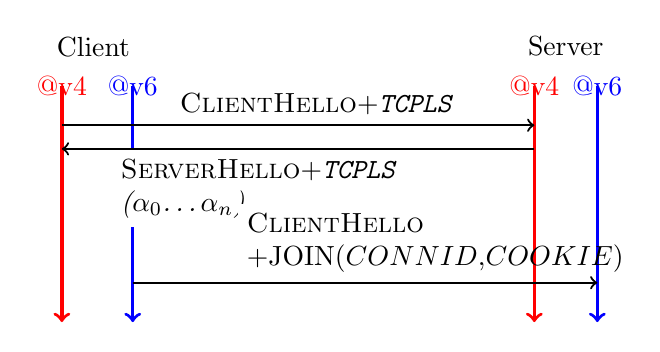
\begin{tikzpicture}
    \colorlet{lightgray}{black!20}
    \tikzstyle{arrow} = [thick,->,>=stealth]
    \tikzset{state/.style={rectangle, dashed, draw, fill=white} }
    \node[black, fill=white] at (0,10) {Client};
    \node[black, fill=white] at (6,10) {Server};
    \node[red, fill=white] at (5.6,9.5) {@v4};
    \node[blue, fill=white] at (6.4,9.5) {@v6};
    \node[red, fill=white] at (-0.4,9.5) {@v4};
    \node[blue, fill=white] at (0.5,9.5) {@v6};
    \draw[red, very thick,->] (-0.4,9.5) -- (-0.4,6.5);
    \draw[blue, very thick,->] (0.5,9.5) -- (0.5,6.5);
    \draw[red, very thick,->] (5.6,9.5) -- (5.6,6.5);
    \draw[blue, very thick,->] (6.4,9.5) -- (6.4,6.5);
   \draw[black, thick, ->] (-0.4,9) -- (5.6,9) node [midway, fill=white, above,
   text width=3cm] {\textsc{ClientHello}+\emph{\tcpls}};
   \draw[black, thick, <-] (-0.4,8.7) -- (5.6,8.7) node [midway, fill=white, below, text width=4.5cm] {\textsc{ServerHello}+\emph{\tcpls($\alpha_0$\ldots$\alpha_n$)} };
   \draw[black, thick, ->] (0.5,7) -- (6.4,7) node [midway, fill=white, above,
   text width=3cm] {\textsc{ClientHello}\\+JOIN($CONNID$,$COOKIE$)};
  \end{tikzpicture}
  \caption{\tcpls supports the attachment of additional \tcp
    connections to a \tcpls connection. Each $\alpha_i$ is encrypted with the
    handshake key.}
  \label{fig:join-example}
\end{figure}
\paragraph*{How to Join}

\tcpls securely solves this \texttt{``connection join''} problem. For example,
consider a client connecting to a dual-stack server. Fig.~\ref{fig:join-example}
depicts the \tls messages exchanged.  The client starts with a
\textsc{ClientHello}. This includes the \tcpls extension to negotiate \tcpls.
The server replies with a \textsc{ServerHello} containing several important and
encrypted control information $\alpha$. First, the server announces its IPv4 and
IPv6 addresses. Second, it associates one connection identifier.  This
identifier uniquely identifies the connection on the server. Third, the server
provides a list of cookies that enable the client to attach additional \tcp
connections to the \tcpls connection. To attach a new connection, e.g., using
the server's IPv6 address, the client opens a \tcp connection and sends a
\textsc{ClientHello} message containing the connection identifier ($CONNID$) and
one of the cookies supplied ($COOKIE$) by the server.

The Connection identifier allows the server to attach the new \tcp connection to
the right \tcpls session, assuming the received cookie is valid. The Connection
identifier and the cookie play that same role as \mptcp's token. However, the
cookie is longer, encrypted in the initial \textsc{ServerHello} message, and
one-time use (i.e., when the server receives a valid cookie, it accepts the
connection, attaches it to the right \tcpls session, and discard the cookie).
Thanks to the cookies, the server can limit the number of \tcp connections that
a client can attach to a \tcpls connection. This prevents some denial-of-service
attacks that are possible with \mptcp.

\subsection{Secure Connection Closing}



%\fr{JOIN is explained here =)}
%Figure~\ref{fig:connmigr} shows a closer look to the \tcpls handshake, and to a
%mpjoin handshake. If the server supports \tcpls, it announces its \tcpLS Encrypted
%Extensions containing the \tcpls connection id \texttt{CONNID}, the list of
%available v4 and v6 addresses from which the sever may be reached, a list of
%one-time use cookies for mpjoin handshakes and lightweight \tcp options. A mpjoin
%handshake is carried out by calling again the \texttt{tcpls\_handshake()} with
%configured handshake properties. This handshake produces a ClientHello with a
%\texttt{JOIN} extension containing information such as the RTT of this
%connection, the \texttt{CONNID} to let the server knows to which \texttt{\tcpls}
%connection bind this \tcp connection, and a \texttt{COOKIE} which acts as an
%authentication mechanism. Note that on-path attackers cannot replay cookies,
%as they are one-time use. However, they can drop the legitimate \texttt{JOIN}
%ClientHello and send the cookie to join the \tcpls's context. The server will
%never send data through a path that has not been confirmed. Confirmation happens
%with a path challenge similar to QUIC, which an on-path attacker in not
%able to answer.

%%\begin{figure}
  %%\begin{tikzpicture}
    %%\colorlet{lightgray}{black!20}
    %%\tikzstyle{arrow} = [thick,->,>=stealth]
    %%\tikzset{state/.style={rectangle, dashed, draw, fill=white} }
    %%\node[black, fill=white] at (0.5,10) {Sender};
    %%\node[black, fill=white] at (6,10) {Receiver};
    %%\node[red, fill=white] at (5.6,9.5) {@v4};
    %%\node[blue, fill=white] at (6.4,9.5) {@v6};
    %%\draw[very thick,->] (0.5,9.5) -- (0.5,0.7);
    %%\draw[red, very thick,->] (5.6,9.5) -- (5.6,0.7);
    %%\draw[blue, very thick,->] (6.4,9.5) -- (6.4,0.7);
    %\node[fill=white] at (0,9) {tcpls\_handshake()};
    %\node[fill=white] at (6,9) {tcpls\_handshake()};
   %\draw[black, thick, ->] (0.5,8) -- (5.6,8) node [midway, fill=white, above,
   %text width=3cm]
   %{Client Hello\\+ extension \tcpls};
   %\draw[black, thick, <-] (0.5,7.7) -- (5.6,7.7) node [midway, fill=white, below,
   %text width=4.5cm] { Server Hello + extension
     %\tcpls+\{CONNID\} + \{ADD\_ADDRS\} + \{COOKIES\} + \{\tcp options\}};
   %\node[fill=white, text width=3cm] at (0.5, 5.5) {Let's migrate on the received
     %v6 addr};
   %\node[fill=white, text width=3cm] at (0.5, 4.5) {tcpls\_handshake()};
   %\draw[black, thick, ->] (0.5,4) -- (6.4,4) node [midway, fill=white, above,
   %text width=3cm]
   %{Client Hello\\+JOIN(CONNID, COOKIE)};
   %\node[fill=white, align=right] at (6.8, 4)
   %{accept()};
   %\node[fill=white, align=right] at (6.1, 3.2)
   %{tcpls\_new()\\tcpls\_handshake()\\tcpls\_accept()};
   %\node[fill=white] at (6.1, 1.9) (Callback) {CB mpjoin!};
   %\node at (7.1, 1.7) (here) {};
   %\draw [->] (Callback) to[out=-80, in=-90,looseness=1.3] (here)
   %to[out=90,in=80,looseness=1.5] (Callback);
   %\node[align=right,fill=white] at (0, 2.5)
   %{tcpls\_stream\_new()\\tcpls\_streams\_attach()\\tcpls\_stream\_close(v4)\\tcpls\_send(v6)};
   %\draw[black, thick, ->] (0.5, 1.2) -- (6.4, 1.2) node [midway, above, text
   %width=3cm] {\{APPDATA\}...\{\tcpls DATA\}...\{APPDATA\}};
  %\end{tikzpicture}
  %\caption{Messages exchanged during an application-level connection migration
    %using \tcpls's API}
  %\label{fig:connmigr}
%\end{figure}


%\begin{figure}
  %\begin{tikzpicture}
    %\colorlet{lightgray}{black!20}
    %\tikzstyle{arrow} = [thick,->,>=stealth]
    %\tikzset{state/.style={rectangle, dashed, draw, fill=white} }
    %\node[black, fill=white] at (0.5,10) {Client};
    %\node[black, fill=white] at (6,10) {Server};
    %\node[red, fill=white] at (5.6,9.5) {@v4};
    %\node[blue, fill=white] at (6.4,9.5) {@v6};
    %\draw[very thick,->] (0.5,9.5) -- (0.5,-2);
    %\draw[red,very thick,->] (6,9.5) -- (6,-2);
    %\draw[blue,very thick,->] (6.2,9.5) -- (6.2,-2);
%%    \node[fill=white] at (0,9) {tcpls\_handshake()};
%%    \node[fill=white] at (6,9) {tcpls\_handshake()};
   %\draw[black, thick, ->] (0.5,8) -- (6,7.5) node [midway, fill=white, above, text width=4cm]
   %{\begin{tabular}{l}SYN\\ClientHello[\tcpls]\end{tabular}};
   %\draw[black, thick, <-] (0.5,7) -- (6,7.5) node [midway, fill=white, below, text width=6cm] {\begin{tabular}{l}SYN+ACK ServerHello[\tcpls(id=123,\\ADDRS(@v4,@v6),C=abc,\ldots)]\end{tabular}};
%%   \node[fill=white, text width=3cm] at (0.5, 4) {Let's migrate on the received
%%     v6 addr};
%%   \node[fill=white, text width=3cm] at (0.5, 3) {tcpls\_handshake()};
   %\draw[black, thick, ->] (0.5,2.5) -- (6.2,2) node [midway, fill=white, above, text width=4cm]
   %{\begin{tabular}{l}SYN,\\ClientHello[JOIN(id=123,C=abc)]\end{tabular}};
%%   \node[fill=white, align=right] at (6.8, 2.5)
%%   {accept()};
%%   \node[fill=white, align=right] at (6.1, 1.7)
%%   {tcpls\_new()\\tcpls\_handshake():};
%%   \node[fill=white] at (6.1, 0.8) (Callback) {CB mpjoin!};
%%   \node at (7.1, 0.6) (here) {};
%%   \draw [->] (Callback) to[out=-80, in=-90,looseness=1.3] (here)
%%   to[out=90,in=80,looseness=1.5] (Callback);
%   \node[fill=white] at (0, 1) {tcpls\_send(on\_v6addr);};
%   \draw[black, thick, ->] (0.5, 0) -- (6, 0) node [midway, above, text
%   width=3cm] {\{APPDATA\}...\{\tcpls DATA\}...\{APPDATA\}};
  %\end{tikzpicture}
%\end{figure}


%-----------------------
\section{\tcpls Prototype[BUDGET=2.5p]}
\label{sec:prototype}
%------------------------
% !TEX root = ./paper.tex
\label{sec:content}

In this section, we describe our \tcpls implementation which provides the 
following benefits.
($i$, \textit{Section \ref{sec:prot-multiplexing}}) Applications can use 
parallel 
streams with 
different cryptographic 
contexts and multiplex them over a \tcp connection.
%(mp): TODO reintegrate this whenever the API has substantial text in the body of the paper
%($ii$) An experimental API that wraps \tls and \tcp and enables applications to
%    handle multihoming, multipathing, and various transport layer mechanisms.
%\todo{MP: mettre la ref du workshop et ne pas expliquer}
($ii$) \tcp options can be sent through the secure \tcpls records, improving 
the extensibility of \tcp. We presented this service in a workshop
paper~\cite{rochet2020tcpls} by implementing the \tcp User Timeout option.
%(as described in
   %Section~\ref{sec:background-design})
   %. We demonstrate this possibility by
   %implementing the \tcp User Timeout option%, which is a building block for
   %our Failover protocol
   %.
   %(mp): TODO move this to a section describe secure TCP options, with maybe 
   %the exchange of eBPF code somehow
   % Supporting another \tcp option is only a matter of
   %extending the sender's API and processing the option on the receiver side.
   %\tcpls's internal machinery allows to the server (resp. client) to send any
   %TCP option during (resp. after) the \tls handshake.
($iii$, \textit{Section \ref{sec:prot-migration}}) Applications can trigger 
Connection Migration and enable Failover.
($iv$, \textit{Section \ref{sec:prot-multipath}}) Applications can leverage 
multipath 
capabilities such as stream 
steering %over several \tcp connections 
and bandwidth aggregation.
%\todo{MP: en faire une petite section qui présente l'implémentation, a 
%combiner p-ê avec (ii)}
($v$, \textit{Section \ref{sec:prot-ebpf}}) The server can securely send eBPF 
bytecode to the client 
to upgrade its \tcp congestion control scheme or tune other \tcp 
mechanisms~\cite{brakmo2017tcp,tran2019beyond}. Through these examples,
%hopefully demonstrate how interesting \tcpls's design can be.
we demonstrate that our design enables modern transport services.

%Variable-length options (e.g., eBPF bytecode) can be sent within streams to 
%take advantage of bandwidth aggregation or Failover when these features are 
%enabled.
%($v$) Different connection migration modes: Failover and Application-level
%Connection Migration.
Our prototype is a fork of the \texttt{picotls} \tls 1.3 implementation 
to which we added 9k lines of C code to implement TCPLS.

\subsection{Multiplexing}
\label{sec:prot-multiplexing}

We leverage the \tcpls records and the \tcpls stream cryptographic contexts to 
build our prototype with a zero-copy receive path. When a record is received,
\tcpls first finds the corresponding cryptographic context, i.e. the
corresponding \tcpls stream for which the derived IV leads to a successful
authentication of the tag. At this stage, prior to full decryption, the 
\tcpls stream of the record is known. Our prototype can then locate the 
corresponding buffer
to perform full decryption at the expected offset without any extra copy.
Applications can benefit from large contiguous
buffers to perform reads instead of receiving stream data on a per-packet basis,
as often found in QUIC implementations.

%\fr{I don't want to give the impression that everything works like a charm -- I
%would need 1 more year to have something production ready}
%We stress that all of these features have been tested but this prototype is a
%research-level implementation. The implementation can
%showcase those features but is however not yet ready for production, as many
%bugs likely remain despite our unit tests and integration tests. Portability was
%neither part of our goals, but might be necessary for a production ready \tcpls
%library.

%\subsection{The \tcpls API}
%
%\todo{(mp): How important is this for conext, rather than IETF? I feel like 
%the subsection content is too thin to have any weight}
%
%The API that applications use to interact with a protocol plays an important
%role in leveraging all the protocol features. The most popular
%API to interact with the transport layer remains the BSD socket API. 
%Researchers
%and the IETF have explored new ways to expose a transport
%API~\cite{draft-ietf-taps-arch,hruby2014sockets,rfc6458,schmidt2013socket}.
%Due to space limitations, we provide in appendix~\ref{appendix:api} a simple 
%example of our API workflow,
%which builds upon good practices proposed by the outlined research.

%In this spirit, application-level developers would only be required to
%configure a \tcpls context and register function callbacks.
%We design \tcpls such
%that the application-level developers can ignore any notion of Network IPC as
%defined by, for example, the POSIX API, the Berkeley socket API or Winsock,
%facilitating application-level development by offering a more concrete
%session-level interface based on asynchronous network events.
%The overall idea is to offer to application developers the opportunity to tune
%the transport protocol for a better usage of the network from their own
%application protocol, which might depend on its distinguishing
%features.
%\todo{we need to explain the mpjoin}


%Note, those features are not stable yet, and many bugs remain to be fixed.

\subsection{Failover}
\label{sec:prot-migration}

%\textbf{Failover}.
We leverage the \tcpls records to securely exchange the \tcp User Timeout option.
This option enables endpoints to detect blackholed and failed \tcp connections
after a given time threshold. We use this as one trigger of the Failover. The 
sender configures this time threshold at the receiver side by sending this \tcp 
option in a \tcpls record. The receiver can then notice when it stops receiving 
data and trigger the Failover.
Receiving a \tcp \texttt{RST} or \texttt{FIN} over a \tcp connection for which
\tcpls streams are attached does also trigger the Failover.

The stream-level acknowledgments required for the Failover to detect the lost
\tcpls records can be enabled at the start of a \tcpls session. The default
policy is to acknowledge every 16 received records, or when a
stream has processed 
%more than $249600$ 
%\todo{Maybe explain the number?}
a given amount of 
bytes since the last acknowledgment. 

Our prototype handles failover over IPv4 and IPv6 \tcp connections, and by default, chooses different source and destination addresses than the failed \tcp connection if possible.

Application running on more constrained devices can choose to disable Failover
to gain in performance. They can also enable Failover during a \tcpls session 
by sending a message on the secure channel. 
We evaluate the performance impact of Failover in 
Section~\ref{sec:eval_failover}

%\textbf{Application Connection Migration}.
%\todo{Is there something to write implementation-wise?}

\subsection{Multipath}
\label{sec:prot-multipath}

\textbf{Stream steering}.
\tcpls exposes the \tcp connections it manages to the application. This allows 
the application to directly distribute the \tcpls streams over the \tcp 
connections at any point of the \tcpls session. A simple distribution is to 
move all \tcpls streams from one connection to another, as performed during 
Application-triggered Connection Migration. Our prototype enable these 
operations in a few API calls. More complex stream attachment policies can be 
implemented by the application to meet its requirements.
%The application, using our \tcpls API can create, attach and steer data within
%any \tcp connection previously created using  \texttt{tcpls\_connect()} and 
%joined using
%\texttt{tcpls\_handshake()}. Properties over the streams can be negotiated, 
%such as the
%failover mode (global to all streams) or \textit{Coupled Streams}, that let the
%application uses the same interface \texttt{tcpls\_send()}  and 
%\texttt{tcpls\_receive()}
%independently of the negotiated stream features. As a matter of example, Stream
%steering and \textit{Coupled Streams} can offer the application to steer a
%connection migration (so called Application Connection Migration in
%section~\ref{sec:transport-services}) in four API calls (i.e., creating a \tcp
%connection, joining the \tcpls session, creating a stream and closing previous
%streams).

\textbf{Bandwidth Aggregation}.
The application can create and join several \tcp connections to
the same \tcpls session. When coupled streams are attached to
different \tcp connections, \tcpls adds a sequence number encrypted in the \tls 
record payload. It is used to reorder the received records 
after decryption. Our prototype only supports coupling all streams together.
%, but
%we envision for the \tcpls protocol to have streams potentially detached from
%the global orderings. 
%For example, a HTTP application may want to use an
%aggregation mode for 2 streams over 2 \tcp connections downloading a video
%content for the video playback engine, but the other streams used by the HTTP
%client do not necessarily need to be part of the multipath bandwidth 
%aggregation.
%Such a feature may be implemented through a negotiation of the aggregation 
%mode.
The sending application implements the scheduling coupled streams over the 
different \tcpls connections.
Our implementation currently includes a round-robin scheduler on the receiver
side. We expect to
support other schedulers in the future and allow the application to select its 
preferred scheduler through the API, or even send it as eBPF bytecode over the 
session. The more \tcpls receives records in order, the more it can deliver 
them in a zero-copy fashion to the application. When a record is received 
out-of-sequence, its content is pushed on an efficient reordering heap. %in 
%$O(log(n))$ for $n$ elements in the heap. Checking the minimum sequence number 
%in the heap is in $\Theta(1)$ and retrieving is in $O(log(n))$. 
The performance of our multipath bandwidth aggregation is evaluated in
Sec.~\ref{sec:bwaggr}.

%\subsubsection{Failover}\label{failover}
%Failover is a binary mode (on/off) that is fully internal to \tcpls.
%Once activated, \tcpls exchanges acknowledgments for records received on each
%stream. These acknowldgments are stream-based and configurable. The default
%acknowledgment policy is to acknowledge every 16 received records, or when a
%stream has processed more than $249,600$ bytes since the last acknowledgment.
%When a \tcp connection conveying \tcpls streams suffers from a network outage (e.g., a \rst is received or the connection becomes idle for too long), we move the stream to a new \tcp connection, retransmit the unacked records, and resume the transfer. Our prototype handles failover over IPv4 and IPv6 \tcp connections, and by default, chooses different source and destination addresses than the failed \tcp connection if some are available.
%%Failover might be negotiated by both party, or
%%enabled by default by both party.
%Depending on the application type, Failover might be enabled or not by 
%default. It is also possible to activate Failover during a \tcpls session by 
%sending a message on the secure channel. We evaluate the performance of 
%Failover in Section~\ref{sec:eval_failover}

%\subsubsection{Application-level Connection Migration}
%\label{sec:connmigr}


%When an application feels right to migrate its connection, it
%can follow those simple steps: activating the multipath aggregation
%mode, then making a \tcpls join handshake on the new path. Then, opening a new stream
%and attaching it to the new \tcp connection, and closing the initial
%stream would make the data transfert enter in a temporary two-paths aggregated mode in
%which the other peer's first path flushes its data if any, and then gracefully close the \tcp
%connection achieving a smooth migration. In practice, such a migration would
%achieve better goodput than a QUIC single-path migration design in which the
%data path is temporally broken and then recovered. In our design, the
%application can make such a migration in 5 API calls.

%\subsection{TCP Options and Kernel extensibility}

\subsection{eBPF code remote attachment}
\label{sec:prot-ebpf}

Recent work on restructuring congestion control has proposed a generic 
architecture for congestion controllers~\cite{narayan2018restructuring}.
Linux kernel developers have relied on eBPF to make the Linux TCP/IP 
stack easier to extend~\cite{brakmo2017tcp,tran2020beyond}. Since Linux kernel 
version 5.6, an application can attach congestion control schemes 
entirely implemented in eBPF. A broader approach was proposed for \quic in 
Pluginizing \quic~\cite{de2019pluginizing}. 
%We leverage these new eBPF capabilities to demonstrate the feasibility of 
%injecting a new congestion control scheme during a \tcpls session.

Our \tcpls prototype enables the server %to use \tcpls streams 
to attach a new eBPF congestion controller to the client over the \tcpls 
session. The type of eBPF code 
that can be attached could be easily extended to other points of the TCP 
execution path.
The eBPF code is conveyed securely in a dedicated \tcpls record. When 
the code is larger than a single \tls record, it can be chunked in several 
records and sent using a \tcpls stream cryptographic context. This service 
illustrates how the flexibility of \tcpls record and streams can be leveraged 
to implement novel transport mechanisms.

%The \tcpls streams enable new use cases. A \tcpls application can
%create and use different streams to carry data. However, since these streams
%are generic, they can also be used by the \tcpls implementation itself to
%exchange control information. To demonstrate the versatility of these control
%streams, we extended \tcpls to enable a server to push a different congestion
%control scheme to a specific client over an existing \tcpls session. 
\subsection{\tcpls Session Establishment}

Our prototype is fully compatible with \tls 1.3 0-RTT session resumption
and \tcp Fast Open option (TFO)~\cite{radhakrishnan2011tcp}. By combining them,
the \tcpls handshake can be sent together with the \tcp \texttt{SYN} starting 
the three way handshake. This provides a low-latency and secure connection establishment.
It is not enabled by default in \tcpls, as TFO trades off some privacy~\cite{sy2020enhanced}.
More advanced techniques such as \tcp Fast Open Privacy~\cite{sy2020enhanced} 
could be
integrated into \tcpls to solve this issue.

%One notable feature of \quic is its ability to establish a secure connection within one round-trip-time with a new server. For subsequent connections with the same server, \quic can even include data during the handshake.

%\tls 1.3 also includes a fast handshake for subsequent connections. When used with \tcp Fast Open (TFO)~\cite{radhakrishnan2011tcp}, the \tls handshake can be sent together with \tcp's three way handshake. However, TFO suffers from privacy issues~\cite{sy2020enhanced}. For this reason, we did not enable it by default in \tcpls. We could revise this decision if a solution similar to \tcp
%FOP~\cite{sy2020enhanced} is included in mainline TCP implementations.


%One argument for QUIC's usage on the web was its first 1-rtt secure connection.
%Compared to TLS/TCP, QUIC has only one handshake and can then proceed with the
%application data. $TLS/TCP$ has two: First, the \tcp three-way handshake, and
%then the \tls handshake.

%\tcpls can use \tcp's TFO~\cite{radhakrishnan2011tcp}
%and send the \texttt{ClientHello} message within the \tcp SYN's payload,
%achieving the same roundtrips than QUIC. However, TFO suffers from privacy
%issues~\cite{sy2020enhanced}, thus we did not enable it by default. In the
%future, we may expect to revise our choice if a solution similar to \tcp
%FOP~\cite{sy2020enhanced} gets implemented in the Linux kernel.



\section{\tcpls Evaluation[BUDGET=3p]}
\label{sec:evaluation}
% !TEX root = ./paper.tex



\subsection{Methodology}

Our objective is to evaluate whether our design and implementation are indeed
fast, flexible and does not conflict with several commercial and open-source
middleboxes. Moreover, we expect to showcase and compare TCPLS's functionalities
such as the App-level connection migration, the failover mechanism or the
bandwidth aggregation capability. We discuss them against the state
of the art designs, such as mvfst~\cite{mvfast}, quicly~\cite{quicly},
msquic~\cite{msquic}, MPTCP~\ref{mptcp}, pquic~\cite{pquic},
quic-go~\cite{quic-go} and MPQUIC~\ref{mpquic}.

%TODO do we also evelatuate security? with a simple proof and discussion?
To evaluate the performance (Section~\ref{sec:perf}) and middlebox traversal
(Section~\ref{sec:middlebox}), we deploy a testbed composed of three machines with Intel Xeon CPU E5-2630
2.40GHz, 16 Threads, at least 16GB RAM, running Debian with 5.9 and
5.7 kernels. Two of these machines play the role of Client and Server,
while one is the Network Simulator (NS). Each machine is equipped with an
Intel XL710 2x40GB NIC, directly connected as shown in
Fig.~\ref{fig:perf_testbed}.
Each device is configured to maximize its performances, with a single TCP connection
reaching 22 Gbps with a 1500 Bytes MTU and linerate (i.e., 40 Gbps) when
using jumbo frames.

\begin{figure}[!t]
  \begin{center}
    \includegraphics[width=6cm]{figures/testbed.png}
  \end{center}
  \vspace{-0.5cm}
  \caption{Performance Measurements Setups. C = Client. S = Server. MB = Middlebox.}
  \label{fig:perf_testbed}
    \vspace{-0.5cm}
\end{figure}

The traffic exchanged by client and server has to go through the NS first.

To evaluate TCPLS's functionalities, we rely on reproducible network
experimentations with Mininet~\cite{mininet}. Our objective is to compare the
behaviour of TCPLS with the state of the art, and to make it easily
reproducible for future works, as the quic implementations continue to evolve.

\subsection{Capability Comparison}

Table~\ref{table:tcplsvsquic} compares the features supported by
\tcp, \tls/\tcp, QUIC and \tcpls. QUIC and \tcpls are very similar in their
capabilities. They mainly differ in their semantic. \tcpls's semantic is to let
the applications make the decision, and we design its API to fulfill this goal.
That is, the meaning of \tcpls is to offer advanced, extensible and secure
transport-layer functionalities on top of \tcp, while exposing a simple but
powerful API to let the application composes the properties its transport should
have.

Note that several of the features suggested by \tcpls are also suggested on \tcp or
QUIC via research works such as a new socket API for explicit multipath for
\tcp\cite{hesmans2016enhanced}, or eBPF plugins in
QUIC~\cite{de2019pluginizing}.

\begin{table}
  \small
  \begin{tabular}{lcccc}
    \toprule
    & \tcp & \tls/\tcp & QUIC & \tcpls \\
    \midrule
    Transport reliability & \checkmark & \checkmark &
    \checkmark & \checkmark \\
    Message conf. and auth.&  \xmark & \checkmark & \checkmark & \checkmark \\
    Connection reliability (failover) &  \xmark & \xmark & (\checkmark) & \checkmark \\
    0-RTT & \checkmark & (\xmark) & \checkmark  & \checkmark \\
    Session Resumption & \xmark & \checkmark & \checkmark & \checkmark \\
    Connection Migration & \xmark & \xmark & \checkmark & \checkmark \\
    \multicolumn{5}{l}{Application-exposed features} \\
    \hspace{2em} Streams & \xmark & \xmark & \checkmark & \checkmark \\
    \hspace{2em} Happy eyeballs & \xmark & \xmark & \xmark & \checkmark \\
    \hspace{2em} Explicit Multipath & \xmark & \xmark & \xmark & \checkmark \\
    \hspace{2em} App-level Con. migration & \xmark & \xmark & \xmark & \checkmark \\
    \hspace{2em} Pluginization & \xmark & \xmark & \xmark & (\checkmark) \\
    Resilience to HOL blocking & \xmark & \xmark & \checkmark  & \checkmark \\
    Secure Connection Closing & \xmark &  \xmark & \checkmark & \checkmark \\
    \bottomrule
  \end{tabular}
  \caption{Protocol features comparison. (\xmark) means that the feature is
    available, but not straightforward to use. (\checkmark) means that the
  feature is partially available and under development.}
  \label{table:tcplsvsquic}
\end{table}

\subsection{Performance}
\label{sec:perf}

We perform a throughput evaluation of \tcpls and compare it to several major
QUIC implementations: mvfst~\cite{} from Facebook, msquic~\cite{} from Microsoft
and quicly~\cite{} from Fastly. Our choice of QUIC implementations was mainly
influenced by the availability of a client/server perf tool specifically
engineered for a throughput evaluation. A second criterion was the advancement
of the implementation and the quality of the code. We hope to avoid most of the
bugs negatively impacting their results by selecting the QUIC implementation
that show advanced features and testings. A third criterion was the development
language used. \tcpls is written in C, and we prefer to compare it against QUIC
implementation written in a language compiled by clang or gcc. Mvfst, msquic
and quicly meet these criteria. Besides, mvfast and quicly also support generic
segmentation offload, which is a plus for throughput experimentation, since those
implementions would speed up thanks to the offloading UDP segmentation and
checksum computation available on our NICs. We use the implementation's
client/server perf tools as is, exploiting the optional arguments provided
by their interface to increase the throughput but drawing the line there. That
is, we do not change their implementation.

Figure~\ref{fig:perf} shows several interesting results. First, while
offering similar (and more) capabilities than what QUIC is providing today,
\tcpls is also more than twice faster than the strongest evaluated QUIC
implementation (quicly) over CPU limited experimentations. We evaluate \tcpls
in four different settings: with a path mtu of 1500 or 9000, and with failover
enabled or not. The failover functionality is an internal stack feature that
provides session reliability, which increases the number of syscalls that TCPLS
makes by exchanging TCPLS-level record acknowledgments. We currently send an ack
for every 16 received records, or when we receive 15 times the maximum TLS
payload, or when a timer expires. Reducing the frequency would improve
throughput at the price of a slower recovery in case of network failure.

TLS/TCP's experiments uses \texttt{picotls}'s client/server implementation with
the same commit than our initial fork for TCPLS. TLS/TCP's lower performance results
can be explained by the receiving buffer size provided to \texttt{read()}, which
is hardcoded to 16384 bytes. This choice makes the client suffers from
fragmentation and cannot exploit the zero-copy code path provided by the
library, which \tcpls can do with a larger read buffer. At first, we may think
that this is not a fair comparison, however the devil is in the detail. In our
implementation, the application developers cannot touch \texttt{read()}'s
interface. That is, the application developer cannot missuse the relationship
between TLS and TCP by creating fragmented records and doing unecessary copies
to handle those fragments. TCPLS's design and implementation may try to prevent
such fragmentation to happen, by first, having a sufficiently large read buffer
size. Second, by deciphering a record only when we known we received the record
entirely. TLS/TCP record fragmentation is provided by TLS libraries as a
usability feature that spares the application developers to care about TLS
details, at the cost of slower performance. \tcpls allows the application
developers to ignore TLS details without missusing the interface,
which is the reason this comparison is interesting. Moreover, but this has not
yet been implemented, it could be interesting to match the TLS record size to
the congestion window to deliver faster the data to the application whe the
network is under congestion.


\begin{figure}[!t] \begin{center}
    \includegraphics[width=\columnwidth]{figures/perf_analysis.png} \end{center}
  \caption{Throughput measurements of various QUIC stacks, TLS/TCP and TCPLS}
  \label{fig:perf} \end{figure}

\subsection{Middlebox Interferences}

When deploying a novel protocol, different middlebox interferences may arise
depending on the changes introduced in the packets wire image. In this
regard, \tcpls comes with two novel \tls extensions: \tcpls and \join.
We discuss the potential issues and contermeasures below.

If a clients attempts to open a \tcpls to in the presence of a \tls termination
proxy, it sends a ClientHello that includes the \tcpls extension. If the proxy
does not support \tcpls, it replies with a ServerHello message that does not
include the \tcpls extension. From this point, the client implicitely fallback
to \tls, and continues with the handshake.

Certain legacy \tls server implementations are known not to implement the \tls
specification properly and might abort connections when receiving unknown TLS
extensions. Analogous behavior has been observed in overly restrictive stateful
firewalls.  To ensure connectivity in the presence of such policies, \tcpls
implements an explicit fallback mechanism. If a device sends a \tcp \rst in
response to the \tcpls-setup ClientHello, or silently discards it, the client
attempts at negotiating a second non-\tcpls \tls connection, either immediately
or after a timeout. Similarly, a \tcpls \join extension might be blocked on the
path. In this case, the subflow attachment is canceled, and the application
is directly notified to be able to react appropriatly.

We tested \tcpls against several opensource and commercial stateful firewalls
implementations (i.e., pfSense, IPFire, Cisco ASAv) and found no interferences.

\subsection{Bandwidth Aggregation}

\begin{figure}[!t] \begin{center}
    \includegraphics[width=\columnwidth]{figures/aggregate_dual.png}
  \end{center} \caption{Bandwidth aggregation comparison between MPTCP and
    TCPLS.} \end{figure}

\subsection{Application-level migration}

Detailler pourquoi on a besoin du controle applicatif pour la migration, et à
quels cas du monde réels ils s'appliquent


Figure~\ref{fig:conn_migration} shows the result of an Application-level
connection migration demo using the API (i.e., it is left to the
application to decide when to migrate, and we expose a simplistic code flow to
perform it). In this experiment, we use an IPMininet network~\cite{ipmininet, jadin2020educational}
composed of a client and a server with a dual-stack of IPs. One path within the
network is composed of OSPF routers with IPv4 only, and one path is composed of
OSPF6 routers IPv6 only. We configure the bandwidth to 30Mbps, the lowest delay
to the v4 link. Our application
downloads a 60 MB file from a server and migrates to the v6 connection in
the middle of the download.

Triggering the connection migration involves chaining 5 API calls:
first, \texttt{tcpls\_handshake()} configured with handshake properties announcing a JOIN over the v6 connection id. Then, the creation of a new stream
\texttt{tcpls\_stream\_new()} for the v6 connection id, finally followed by the attachment of this new stream \texttt{tcpls\_streams\_attach()} and the secure closing of the v4 \tcp connection using \texttt{tcpls\_stream\_close()}. Following these events, the server seamlessly switches the path while looping over \texttt{tcpls\_send} to send the file content. Note that all the events trigger callbacks on the server side, to let the server react appropriately if other requirements need to be fulfilled.

\tcpls's application connection migration takes advantage of multipath to offer
a smooth handover to applications, which QUIC cannot do at the moment.

\begin{figure}[!t]
  \centering
  \includegraphics[width=6cm]{figures/migration.png}
  \caption{Application-level connection migration during a 60MB file download.}
  \label{fig:conn_migration}
\end{figure}

\subsection{Failover}

1) analyse du temps de recovery pour different type de cassure, et comparaison avec mptcp
2) discuter une propriété de "connection reliability" => ca casse, on restabilise le plus vite possible
3) montrer que le path manager est important pour cette propriété, et que ce n'est pas encore au point pour mptcp, mpquic, etc

Mptcp overhead: 1.0744997978210449
TCPLS overhead: 1.0994282363439873
MPTCP overhead/TCPLS overhead:              0.9773259975513828


\begin{figure}[!t]
  \begin{center}
    \includegraphics[width=6cm]{figures/breakage_analysis.png}
  \end{center}
  \caption{Recovery speed analysis.}
\end{figure}


\begin{figure}[!t]
  \begin{center}
    \includegraphics[width=6cm]{figures/tcpls_mptcp.png}
  \end{center}
  \caption{Connection reliability: influence of the path manager and congestion
  control.}
\end{figure}



\subsection{Dynamically extending TCPLS}

The TCPLS streams enable new use case. Obviously, a TCPLS application can
create and use different streams to carry data. However, since these streams
are generic, they can also be used by the TCPLS implementation itself to
exchange control information. To demonstrate the versatily of these control
streams, we extended TCPLS to enable a server to push a different congestion
control scheme to a specific client over an existing TCPLS session. Recent
work on restructuring congestion control has proposed a generic architecture
for congestion controllers \cite{narayan2018restructuring}. 
During the last years, the Linux kernel developpers have relied on eBPF
to make the Linux TCP/IP stack \cite{brakmo2017tcp,tran2020beyond} easier
to extend. Since Linux kernel version 5.xx, $Emery$ an application can inject
a different congestion control scheme entirely implemented using eBPF. A similar approach was proposed in Pluginizing QUIC~\cite{de2019pluginizing}.
We leverage these new eBPF capabilities to
demonstrate the feasibility of injecting and
updating a congestion control scheme during a TCPLS session.

We perform our experiment using Mininet over a 100 Mbps emulated link that has a 60 msec delay. Figure~\ref{fig:vegasCubic} shows a client that uses the TCP Vegas \cite{10.1145/190314.190317} congestion control scheme to upload a file. This TCLPS session fully uses the bottleneck link. After some time, another client starts an upload, but using the CUBIC congestion controller \cite{rfc8312}. This results in an unfair distribution of the bandwidth. The server then sends the eBPF bytecode of the CUBIC congestion control scheme to the TCP Vegas client that injects it in its kernel and the unfairness disappears.

\begin{figure}[!t]
  \begin{center}
    \includegraphics[width=6cm]{pretty_plotify/plots/vegas_cubic.png}
  \end{center}
  \caption{TCPLS hosts can exchange congestion control schemes and activate them during a TCPLS session.}
  \label{fig:vegasCubic}
\end{figure}











Injecter un control de congestion, montrer que les perf s'améliorent



%-----------------------
\section{Related work}
\label{sec:related}
%------------------------
% !TEX root = ./paper.tex

By closely coupling \tcp and \tls, \tcpls builds upon two of the most important
end-to-end protocols. Given the huge activity on these two protocols within the
research community and the IETF, we restrict our discussion to the closest
related works. Several survey papers provide additional context information
\cite{polese2019survey,li2016multipath,papastergiou2016ossifying}.

Given its security features, \tcpls must be compared with \tcpcrypt
\cite{bittau2010case,rfc8548}. \tcpcrypt predates \tls 1.3. It uses TCP options
to support opportunistic encryption but is not secure against an active network
attacker. \tcpls is compatible with \tls, retains its security properties and supports
additional features. It is also compatible with \tcp middleboxes.

\tcpls also needs to be compared with \mptcp \cite{raiciu2012hard,rfc6824}.
\mptcp supports several coupled congestion control schemes
\cite{peng2014multipath,wischik2011design,khalili2013mptcp} that preserve
fairness even when different paths share the same bottleneck. These are not yet
included in our \tcpls prototype, but could be added with some engineering
effort. The initial idea of coupling \mptcp and \tls was proposed in an expired
Internet draft \cite{draft-paasch-mptcp-ssl-00}, but it was not adopted by the
IETF. MPTCPSec \cite{jadin2017securing} adds security capabilities to \mptcp but
comes with a large performance penalty.

Another important related work is \quic. The initial design
\cite{roskind2013quic} has evolved a lot and large companies have started to
adopt it \cite{langley2017quic,Joras_mvfst,marx2020same}. The \quic
version 1 specification \cite{draft-ietf-quic-transport} supports connection
migration like \tcpls, but we could not test it in our lab since none of the
available open-source implementations have yet implemented it. Multipath
extensions
\cite{viernickel2018multipath,de2017multipath,draft-deconinck-quic-multipath-06,draft-liu-multipath-quic-02}
to \quic have been discussed but not yet adopted within the IETF. Finally, PQUIC
\cite{de2019pluginizing} proposed to carry eBPF code over \quic connections to
deploy new protocol features. This goes beyond the exchange of congestion
control scheme that we demonstrated with \tcpls.

Finally, several solutions have been proposed to provide multipath capabilities
in the application layer. Examples include MP-H2 \cite{nikravesh2019mp} that
extends HTTP/2, MP-DASH \cite{han2016mp} for video streaming or mHTTP
\cite{kim2014multi} that extends HTTP.


\tcpls's idea has also similarities with TLS FOP~\cite{sy2020enhanced}, a
proposal to solve the privacy issue with TFO. However, \tcpls is more generic,
and shows how we can achieve such extensibility work for any other concerns and
new features.

%% Several researchers have proposed techniques to extend various transport
%% protocols. The IETF provides generic guidelines on the design of
%% protocol extensions \cite{rfc6709}. Several researchers have proposed
%% solutions to simplify the implementation of extensions to transport
%% protocols. The closest example include STP \cite{patel2003upgrading}, CTP
%% \cite{bridges2007configurable} and 

%% Patel et al. \cite{patel2003upgrading} propose to use a type-safe version of C to extend a TCP
%% implementation by using bytecode. The implementation of TCPLS completely differs since it uses C to generate eBPF code. Furthemore, by leveraging the
%% flexibility of TLS, TCPLS can securrely exchange various options over a
%% connection. Bridges et al.
%% In CTP, Bridges et al. propose a new protocol that is composed of different microprotocols which can be combined together. In PQUIC, De Coninck et al. \cite{de2019pluginizing} include an eBPF virtual machine inside a QUIC implementation to extend it by using protocol plugins. Our approach is similar from an implementation viewpoint. By combining the TLS and TCP layers, we bring more extensibility to TCP.

%% %maybe
%% % ictcp \cite{wong2001configurable}

%% %configurable and extensible transport \cite{wong2001configurable}

%% % other protocols maybe

%% The IETF has developed various transport protocols, including
%% DCCP \cite{kohler2006designing}, SCTP \cite{rfc4960} and QUIC \cite{draft-ietf-quic-transport}. DCCP brings more flexible congestion control schemes

%% , lots of research but nothing related \cite{nowlan2012fitting}




%% % maybe
%% % Structured streams \cite{ford2007structured}


%% %TCP papers
%% %generic on extensibility

%% %tcp unreliable

%% A wide range of TCP extensions have been proposed \cite{rfc7414}. Some tune
%% protocol implementations with new strategies to retransmit lost data,
%% compute retransmission timers or manage congestion. These do not require
%% the definition of new TCP options that are negotiated during the handshake.
%% Some TCP extensions require the definition of new TCP options. These
%% include the timestamp and large windows extension \cite{rfc7313},
%% the support for selective acknowledgements \cite{rfc2018}, TCP Fast Open
%% \cite{rfc7413} or Multipath TCP \cite{rfc6824}. These extensions are negotiated
%% by exchanging TCP options during the connection handshake. These TCP options
%% allow to extend TCP, but they suffer from several limitations. First,
%% there is limited space in the TCP header to carry them. This limits the
%% number of extensions that can be used for a given TCP connection. The IETF
%% discusses solutions to extend the TCP header space, but the solution is neither
%% finalized nor implemented \cite{draft-ietf-tcpm-tcp-edo-10}. Second, middleboxes
%% interfere with the utilization of new options \cite{honda2011still}. This
%% interference severely limits the extensibility of TCP. TCPLS does not suffer
%% from these problems since the options that it carries are encrypted and can
%% span an entire TLS record (16KBytes).


%% % \cite{nowlan2012fitting}
%% %TODO
%% % idée de combiner des infos de TLS dans MPTCP
%% %\cite{draft-paasch-mptcp-ssl-00}
%% %\cite{jadin2017securing} % secure mptcp


\section{Conclusion[BUDGET=0.5]}
\label{sec:conclusion}
% !TEX root = ./paper.tex
\tcp and \tls were designed as independent protocols, but they are very often
used together. In this paper, we have shown that this is possible to design and
implement the \tcpls protocol that is fast, flexible, and secure by closely
coupling \tcp and \tls.

\tcpls inherits the security features of \tls 1.3 and all the reliability and
congestion control techniques that have been added to \tcp during the last
decades. More specifically, \tcpls extends the \tls 1.3 handshake and the record
layer to create a secure control channel between the two communicating hosts.
The messages exchanged over this channel are placed inside \tls records that are
encrypted and authenticated and also hidden from middleboxes. \tcpls leverages
these control messages to support fast failovers, but also offer smooth
migration of the \tcpls session from one path to another or provide bandwidth
aggregation under full control of the application through an API. \tcpls can
also use the secure channel to extend \tcp with new options and even use the
\tcpls session to exchange a different congestion control scheme that is then
used for this session.

Thanks to \tcpls's design, our \tcpls implementation provides a
flexible API that allows the applications to perform zero-copy data transfers,
and easily manipulate the different features presented in this research work.
Our performance evaluation shows that this prototype is more than twice as fast
as currently available \quic implementations while already supporting additional
features such as bandwidth aggregation and stream steering.

\tcpls is both simple and powerful. Simple because it can be implemented inside
existing \tls libraries without any kernel change in contrast to \tcp. \tcpls is
wire-compatible with the existing \tcp middleboxes and can thus be used in all
environments where \tls is used over \tcp. Given the performance benefits of
\tcpls, the flexibility it offers and the features that it already provides, we
believe it can be a strong contender to \quic for modern services, including
HTTP.



%\section{Implementation, Deployment \& Research Questions}

%
A \texttt{TCPLS} reference implementation is under active development. The
current implementation is forked from a fast and full
TLS 1.3 implementation written in \texttt{C}. It currently adds about 5k lines
of code (including unit tests and inline code comments) compared to the upstream branch.

The current implementation offers: 
\begin{inparaenum}
  \item An experimental API that wraps TLS and TCP
  \item Our design of TCP's extensibility mechanism throught TCP option sent
within TLS records and processed by TCPLS. We currently support TCP User
Timeout and the injection of eBPF bytecode for TCP's congestion control
algorithm. Supporting another TCP option is only a matter of extending the sender's
API and processing the option
on the receiver side. TCPLS's internal machinery is already implemented for any
type of TCP option to send during the handshake or when the handshake completed.
  \item The support of parallel streams and multiplexing over TCP connections.
    Each stream has its own cryptographic context.
  \item Connection migration and multipathing.
\end{inparaenum}

We expect to investigate several research questions with TCPLS. First, we are
interested in analyzing how far we can go into supporting TCP's extensibility
through our mechanism. Several of new TCP features may require to inject eBPF
bytecode to the kernel. It is still unclear how much of TCP could be extended,
and if \texttt{TCPLS} may play a role in incentivizing the linux kernel's maintainer
to support more eBPF in TCP's implementation, since we now offer a technique to
propagate eBPF bytecode within authenticated and confidential session with a
trusted server.

Second, we expect to analyze several features of TCPLS, such as our
connection migration, our multipath implementation and our failover mechanism.
Answering the question about how much TCPLS can or and how fast it performs in
case of a migration or a network outage.

Finally, we would expect to critisize QUIC in light of our \texttt{TCPLS}
design. We will compare both QUIC and TCPLS, discuss the differences, and analyze
and answer questions regarding the requirements in transport protocol for today's
Internet applications.





%\section{Related Work}

%% !TEX root = ./paper.tex

By closely coupling \tcp and \tls, \tcpls builds upon two of the most important
end-to-end protocols. Given the huge activity on these two protocols within the
research community and the IETF, we restrict our discussion to the closest
related works. Several survey papers provide additional context information
\cite{polese2019survey,li2016multipath,papastergiou2016ossifying}.

Given its security features, \tcpls must be compared with \tcpcrypt
\cite{bittau2010case,rfc8548}. \tcpcrypt predates \tls 1.3. It uses TCP options
to support opportunistic encryption but is not secure against an active network
attacker. \tcpls is compatible with \tls, retains its security properties and supports
additional features. It is also compatible with \tcp middleboxes.

\tcpls also needs to be compared with \mptcp \cite{raiciu2012hard,rfc6824}.
\mptcp supports several coupled congestion control schemes
\cite{peng2014multipath,wischik2011design,khalili2013mptcp} that preserve
fairness even when different paths share the same bottleneck. These are not yet
included in our \tcpls prototype, but could be added with some engineering
effort. The initial idea of coupling \mptcp and \tls was proposed in an expired
Internet draft \cite{draft-paasch-mptcp-ssl-00}, but it was not adopted by the
IETF. MPTCPSec \cite{jadin2017securing} adds security capabilities to \mptcp but
comes with a large performance penalty.

Another important related work is \quic. The initial design
\cite{roskind2013quic} has evolved a lot and large companies have started to
adopt it \cite{langley2017quic,Joras_mvfst,marx2020same}. The \quic
version 1 specification \cite{draft-ietf-quic-transport} supports connection
migration like \tcpls, but we could not test it in our lab since none of the
available open-source implementations have yet implemented it. Multipath
extensions
\cite{viernickel2018multipath,de2017multipath,draft-deconinck-quic-multipath-06,draft-liu-multipath-quic-02}
to \quic have been discussed but not yet adopted within the IETF. Finally, PQUIC
\cite{de2019pluginizing} proposed to carry eBPF code over \quic connections to
deploy new protocol features. This goes beyond the exchange of congestion
control scheme that we demonstrated with \tcpls.

Finally, several solutions have been proposed to provide multipath capabilities
in the application layer. Examples include MP-H2 \cite{nikravesh2019mp} that
extends HTTP/2, MP-DASH \cite{han2016mp} for video streaming or mHTTP
\cite{kim2014multi} that extends HTTP.


\tcpls's idea has also similarities with TLS FOP~\cite{sy2020enhanced}, a
proposal to solve the privacy issue with TFO. However, \tcpls is more generic,
and shows how we can achieve such extensibility work for any other concerns and
new features.

%% Several researchers have proposed techniques to extend various transport
%% protocols. The IETF provides generic guidelines on the design of
%% protocol extensions \cite{rfc6709}. Several researchers have proposed
%% solutions to simplify the implementation of extensions to transport
%% protocols. The closest example include STP \cite{patel2003upgrading}, CTP
%% \cite{bridges2007configurable} and 

%% Patel et al. \cite{patel2003upgrading} propose to use a type-safe version of C to extend a TCP
%% implementation by using bytecode. The implementation of TCPLS completely differs since it uses C to generate eBPF code. Furthemore, by leveraging the
%% flexibility of TLS, TCPLS can securrely exchange various options over a
%% connection. Bridges et al.
%% In CTP, Bridges et al. propose a new protocol that is composed of different microprotocols which can be combined together. In PQUIC, De Coninck et al. \cite{de2019pluginizing} include an eBPF virtual machine inside a QUIC implementation to extend it by using protocol plugins. Our approach is similar from an implementation viewpoint. By combining the TLS and TCP layers, we bring more extensibility to TCP.

%% %maybe
%% % ictcp \cite{wong2001configurable}

%% %configurable and extensible transport \cite{wong2001configurable}

%% % other protocols maybe

%% The IETF has developed various transport protocols, including
%% DCCP \cite{kohler2006designing}, SCTP \cite{rfc4960} and QUIC \cite{draft-ietf-quic-transport}. DCCP brings more flexible congestion control schemes

%% , lots of research but nothing related \cite{nowlan2012fitting}




%% % maybe
%% % Structured streams \cite{ford2007structured}


%% %TCP papers
%% %generic on extensibility

%% %tcp unreliable

%% A wide range of TCP extensions have been proposed \cite{rfc7414}. Some tune
%% protocol implementations with new strategies to retransmit lost data,
%% compute retransmission timers or manage congestion. These do not require
%% the definition of new TCP options that are negotiated during the handshake.
%% Some TCP extensions require the definition of new TCP options. These
%% include the timestamp and large windows extension \cite{rfc7313},
%% the support for selective acknowledgements \cite{rfc2018}, TCP Fast Open
%% \cite{rfc7413} or Multipath TCP \cite{rfc6824}. These extensions are negotiated
%% by exchanging TCP options during the connection handshake. These TCP options
%% allow to extend TCP, but they suffer from several limitations. First,
%% there is limited space in the TCP header to carry them. This limits the
%% number of extensions that can be used for a given TCP connection. The IETF
%% discusses solutions to extend the TCP header space, but the solution is neither
%% finalized nor implemented \cite{draft-ietf-tcpm-tcp-edo-10}. Second, middleboxes
%% interfere with the utilization of new options \cite{honda2011still}. This
%% interference severely limits the extensibility of TCP. TCPLS does not suffer
%% from these problems since the options that it carries are encrypted and can
%% span an entire TLS record (16KBytes).


%% % \cite{nowlan2012fitting}
%% %TODO
%% % idée de combiner des infos de TLS dans MPTCP
%% %\cite{draft-paasch-mptcp-ssl-00}
%% %\cite{jadin2017securing} % secure mptcp


%\section{Discussion}

%\input{discussion}


\newpage

\section*{Software Artefacts}
%\todo{BD: this section breaks the submission anonymity.  I would, at this step, only considered what I have written in the intro.}

We will release a detailed description of \tcpls and a reference implementation
together with the camera-ready version of the paper. To preserve anonimity,
we cannot provide additional details here. 

%is under active development. The
%current specifications and code are available on
%\url{https://pluginized-protocols.org/tcpls}, forked from a fast and
%full TLS 1.3 implementation written in \texttt{C}. Our \tcpls prototype adds
%about 5k lines of C code to \texttt{picotls} latest version based on the latest
%specification of TLS 1.3.

%\section*{Acknowledgments}
%We thanks the anonymous reviewers for their helpful feedback, and Mathieu Jadin
%for its helpful guidance with IPMininet. This research is supported by the Walloon
%Region through the ``Programme de recherche d'interet general
 %WALINNOV" - MQUIC project (convention number 1810018).


\bibliographystyle{ACM-Reference-Format}
\bibliography{reference}

\appendix
\label{sec:appendices}

% !TEX root = ./paper.tex

\section{Capability Comparison}

Table~\ref{table:tcplsvsquic} compares the features supported by
\tcp, \tls/\tcp, \quic and \tcpls. \quic and \tcpls are very similar in their
capabilities. They mainly differ in their semantic. \tcpls's semantic is to let
the applications make the decision, and we design its API to fulfill this goal.
That is, the meaning of \tcpls is to offer advanced, extensible and secure
transport-layer functionalities on top of \tcp, while exposing a simple but
powerful API to let the application composes the properties its transport should
have.

Note that several of the features suggested by \tcpls are also suggested on \tcp or \quic via research works such as a new socket API for explicit \mptcp \cite{hesmans2016enhanced}, or eBPF plugins in
\quic~\cite{de2019pluginizing}.

\begin{table}[!t]
  \small
  \begin{tabular}{lcccc}
    \toprule
    & \tcp & \tls/\tcp & \quic & \tcpls \\
    \midrule
    Transport reliability & \checkmark & \checkmark &
    \checkmark & \checkmark \\
    Message conf. and auth.&  \xmark & \checkmark & \checkmark & \checkmark \\
    Connection reliability (failover) &  \xmark & \xmark & (\checkmark) & \checkmark \\
    0-RTT & \checkmark & (\xmark) & \checkmark  & \checkmark \\
    Session Resumption & \xmark & \checkmark & \checkmark & \checkmark \\
    Connection Migration & \xmark & \xmark & \checkmark & \checkmark \\
    \multicolumn{5}{l}{Application-exposed features} \\
    \hspace{2em} Streams & \xmark & \xmark & \checkmark & \checkmark \\
    \hspace{2em} Happy eyeballs & \xmark & \xmark & \xmark & \checkmark \\
    \hspace{2em} Explicit Multipath & \xmark & \xmark & \xmark & \checkmark \\
    \hspace{2em} App-level Con. migration & \xmark & \xmark & \xmark & \checkmark \\
    \hspace{2em} Pluginization & \xmark & \xmark & \xmark & (\checkmark) \\
    Resilience to HOL blocking & \xmark & \xmark & \checkmark  & \checkmark \\
    Secure Connection Closing & \xmark &  \xmark & \checkmark & \checkmark \\
    \bottomrule
  \end{tabular}
  \caption{Protocol features comparison. (\xmark) means that the feature is
    available, but not straightforward to use. (\checkmark) means that the
  feature is partially available and under development.}
  \label{table:tcplsvsquic}
\end{table}

\section{Failover Protocol}
% Agents
\def\Client{Client}
\def\Server{Server}
\def\Inactivity{Inactivity}
\def\Event{Event}


\begin{figure}[!t]
 \begin{center}
\begin{tikzpicture}[every node/.style={font=\tiny, minimum height=0.03cm,minimum width=0.03cm},scale=0.90, transform shape]
\tikzset{label/.style={align=center,minimum height=0.5cm,minimum width=5mm}}
\node [matrix, very thin,column sep=2.2cm,row sep=0.05cm] (matrix) at (0,0) {
  & \node(0,0) (\Client) {}; & \node(0,0) (\Inactivity) {};  & \node(0,0) (\Server) {};  & \\
  & \node(0,0) (\Client 0) {}; & & \node(0,0) (\Server 0) {};  & \\
  \node(0,0) (u1 left) {}; & & & &   \node(0,0) (u1 right) {};\\
  \node(0,0) (t0 left) {}; & \node(0,0) (\Client 1) {}; & \node(0,0) (\Event 1) {}; & \node(0,0) (\Server 1) {};  & \node(0,0) (t0 right) {};\\
   \node(0,0) (u1 left) {}; & & & &   \node(0,0) (u1 right) {};\\
 \node[label] (t1 left) {}; & \node(0,0) (\Client 2) {}; & \node(0,0) (\Event 2) {}; & \node(0,0) (\Server 2) {};  &\node(0,0) (t1 right) {}; \\
  \node(0,0) (u2 left) {}; & & & &   \node(0,0) (u2 right) {};\\
\node(0,0) (t2 left) {};  & \node(0,0) (\Client 3) {}; & \node(0,0) (\Event 3) {}; & \node(0,0) (\Server 3) {};  & \node(0,0) (t2 right) {};\\
  \node(0,0) (u3 left) {}; & & & &   \node(0,0) (u3 right) {};\\
  \node(0,0) (t3 left) {}; & \node(0,0) (\Client 4) {}; & \node(0,0) (\Event 4) {}; & \node(0,0) (\Server 4) {};  &  \node(0,0) (t3 right) {};\\
  \node(0,0) (u4 left) {}; & & & &   \node(0,0) (u4 right) {};\\
 \node(0,0) (t4 left) {}; & \node(0,0) (\Client 5) {}; & \node(0,0) (\Event 5) {}; & \node(0,0) (\Server 5) {};  & \node(0,0) (t4 right) {}; \\
  \node(0,0) (u5 left) {}; & & & &   \node(0,0) (u5 right) {};\\
 \node(0,0) (t5 left) {}; & \node(0,0) (\Client 6) {}; & \node(0,0) (\Event 6) {}; & \node(0,0) (\Server 6) {};  & \node(0,0) (t5 right) {};\\
  \node(0,0) (u6 left) {}; & & & &   \node(0,0) (u6 right) {};\\
 \node(0,0) (t6 left) {};  & \node(0,0) (\Client 7) {}; & \node(0,0) (\Event 7) {}; & \node(0,0) (\Server 7) {};  & \node(0,0) (t6 right) {};\\
  \node(0,0) (u7 left) {}; & & & &   \node(0,0) (u7 right) {};\\
 \node(0,0) (t7 left) {}; & \node(0,0) (\Client 8) {}; & \node(0,0) (\Event 8) {}; & \node(0,0) (\Server 8) {};  &  \node(0,0) (t7 right) {}; \\
  \node(0,0) (u8 left) {}; & & & &   \node(0,0) (u8 right) {};\\
  \node(0,0) (t8 left) {}; & \node(0,0) (\Client 9) {}; & \node(0,0) (\Event 9) {}; & \node(0,0) (\Server 9) {};  & \node(0,0) (t8 right) {};\\
  \node(0,0) (u9 left) {}; & & & &   \node(0,0) (u9 right) {};\\
 \node(0,0) (t9 left) {}; & \node(0,0) (\Client 10) {}; & \node(0,0) (\Event 10) {}; & \node(0,0) (\Server 10) {};  & \node(0,0) (t9 right) {};\\
  \node(0,0) (u10 left) {}; & & & &   \node(0,0) (u10 right) {};\\
  \node(0,0) (t10 left) {}; & \node(0,0) (\Client 11) {}; & \node(0,0) (\Event 11) {}; & \node(0,0) (\Server 11) {};  & \node(0,0) (t10 right) {};\\
  \node(0,0) (u11 left) {}; & & & &   \node(0,0) (u11 right) {};\\
  \node(0,0) (t11 left) {}; & \node(0,0) (\Client 12) {}; & \node(0,0) (\Event 12) {}; & \node(0,0) (\Server 12) {};  & \node(0,0) (t11 right) {};\\
   \node(0,0) (t12 left) {}; & & & &   \node(0,0) (t12 right) {};\\
  & \node(0,0) (\Client 13) {}; & \node(0,0) (\Event 13) {}; & \node(0,0) (\Server 13) {};  & \\
   \node(0,0) (u13 left) {}; & & & &   \node(0,0) (u13 right) {};\\
 \node(0,0) (t13 left) {}; & \node(0,0) (\Client 14) {}; & \node(0,0) (\Event 14) {}; & \node(0,0) (\Server 14) {};  &  \node(0,0) (t13 right) {};\\
   \node(0,0) (u14 left) {}; & & & &   \node(0,0) (u14 right) {};\\
 \node(0,0) (t14 left) {}; & \node(0,0) (\Client 15) {}; & \node(0,0) (\Event 15) {}; & \node(0,0) (\Server 15) {};  & \node(0,0) (t14 right) {};\\
   \node(0,0) (u15 left) {}; & & & &   \node(0,0) (u15 right) {};\\
  \node(0,0) (t15 left) {};  & \node(0,0) (\Client 16) {}; & \node(0,0) (\Event 16) {}; & \node(0,0) (\Server 16) {};  & \node(0,0) (t15 right) {};\\
   \node(0,0) (u16 left) {}; & & & &   \node(0,0) (u16 right) {};\\
 \node(0,0) (t16 left) {}; & \node(0,0) (\Client 17) {}; & \node(0,0) (\Event 17) {}; & \node(0,0) (\Server 17) {};  & \node(0,0) (t16 right) {};\\
  \node(0,0) (u17 left) {}; & & & &   \node(0,0) (u17 right) {};\\
 \node(0,0) (t17 left) {};  & \node(0,0) (\Client 18) {}; & \node(0,0) (\Event 18) {}; & \node(0,0) (\Server 18) {};  &\node(0,0) (t17 right) {}; \\
  \node(0,0) (t18 left) {}; & & & &   \node(0,0) (t18 right) {};\\
  & \node(0,0) (\Client 19) {}; & \node(0,0) (\Event 19) {}; & \node(0,0) (\Server 19) {};  & \\
  \node(0,0) (t20 left) {}; & & & &   \node(0,0) (t20 right) {};\\
  & \node(0,0) (\Client 20) {}; & \node(0,0) (\Event 20) {}; & \node(0,0) (\Server 20) {};  & \\
  \node(0,0) (u21 left) {}; & & & &   \node(0,0) (u21 right) {};\\
  \node(0,0) (t21 left) {};& \node(0,0) (\Client 21) {}; & \node(0,0) (\Event 21) {}; & \node(0,0) (\Server 21) {};  & \node(0,0) (t21 right) {};\\
  \node(0,0) (u22 left) {}; & & & &   \node(0,0) (u22 right) {};\\
 \node(0,0) (t22 left) {}; & \node(0,0) (\Client 22) {}; & \node(0,0) (\Event 22) {}; & \node(0,0) (\Server 22) {};  &  \node(0,0) (t22 right) {};\\
  \node(0,0) (u23 left) {}; & & & &   \node(0,0) (u23 right) {};\\
 \node(0,0) (t23 left) {}; & \node(0,0) (\Client 23) {}; & \node(0,0) (\Event 23) {}; & \node(0,0) (\Server 23) {};  & \node(0,0) (t23 right) {};\\
  \node(0,0) (u24 left) {}; & & & &   \node(0,0) (u24 right) {};\\
 \node(0,0) (t24 left) {}; & \node(0,0) (\Client 24) {}; & \node(0,0) (\Event 24) {}; & \node(0,0) (\Server 24) {};  & \node(0,0) (t24 right) {};\\
  \node(0,0) (t25 left) {}; & & & &   \node(0,0) (t25 right) {};\\
  & \node(0,0) (\Client 25) {}; & \node(0,0) (\Event 25) {}; & \node(0,0) (\Server 25) {};  & \\
  \node(0,0) (t26 left) {}; & & & &   \node(0,0) (t26 right) {};\\
  & \node(0,0) (\Client 26) {}; & \node(0,0) (\Event 26) {}; & \node(0,0) (\Server 26) {};  & \\
};

% Agents labels
\fill
	(\Client) node[draw,fill=white] {\Client}
	(\Server) node[draw,fill=white] {\Server};

% Horizontal time lines
\draw [dotted]
  (t0 left) -- (t0 right) node[right] {$72.18ms$}
  (t0 right) -- (t0 left) node[left] {$51.95ms$}
  (t1 left) -- (t1 right) node[right] {$72.87ms$}
  (t1 right) -- (t1 left) node[left] {$96.17ms$}
  (t2 left) -- (t2 right) node[right] {$73.06ms$}
  (t2 right) -- (t2 left) node[left] {$96.72ms$}
  (t3 left) -- (t3 right) node[right] {$73.18ms$}
  (t3 right) -- (t3 left) node[left] {$96.86ms$}
  (t4 left) -- (t4 right) node[right] {$75.85ms$}
  (t4 right) -- (t4 left) node[left] {$96.92ms$}
  (t5 left) -- (t5 right) node[right] {$117.27ms$}
  (t5 right) -- (t5 left) node[left] {$97.07ms$}
  (t6 left) -- (t6 right) node[right] {$117.63ms$}
  (t6 right) -- (t6 left) node[left] {$137.91ms$}
  (t7 left) -- (t7 right) node[right] {$117.71ms$}
  (t7 right) -- (t7 left) node[left] {$139.12ms$}
  (t8 left) -- (t8 right) node[right] {$117.96ms$}
  (t8 right) -- (t8 left) node[left] {$178.22ms$}
  (t11 left) -- (t11 right) node[right] {$289.05ms$}
  (t11 right) -- (t11 left) node[left] {$268.93ms$}
  (t13 left) -- (t13 right) node[right] {$15870.75ms$}
  (t13 right) -- (t13 left) node[left] {$15991.13ms$}
  (t14 left) -- (t14 right) node[right] {$15891.35ms$}
  (t14 right) -- (t14 left) node[left] {$15911.63ms$}
  (t15 left) -- (t15 right) node[right] {$15891.53ms$}
  (t15 right) -- (t15 left) node[left] {$15911.92ms$}
  (t16 left) -- (t16 right) node[right] {$15932.18ms$}
  (t16 right) -- (t16 left) node[left] {$15911.98ms$}
  (t17 left) -- (t17 right) node[right] {$15971.53ms$}
  (t17 right) -- (t17 left) node[left] {$15961.92ms$}
  (t21 left) -- (t21 right) node[right] {$15991.98ms$}
  (t21 right) -- (t21 left) node[left] {$15971.98ms$}
  (t22 left) -- (t22 right) node[right] {$18432.62ms$}
  (t22 right) -- (t22 left) node[left] {$19319.70ms$}
  (t23 left) -- (t23 right) node[right] {$20434.87ms$}
  (t23 right) -- (t23 left) node[left] {$21407.99ms$}
  (t24 left) -- (t24 right) node[right] {$21468.34ms$}
  (t24 right) -- (t24 left) node[left] {$21408.06ms$};

\draw
  (\Client 0)
    node[draw,rectangle,fill=yellow!20, rotate=-90]
      (\Client Timeline In) {}
    node[below right] {}
  (\Server 0)
    node[draw,rectangle,fill=yellow!20, rotate=-90]
      (\Server Timeline In) {}
    node[below right] {};

% Vertical flows
\draw [-latex] (\Client Timeline In.east) -- (\Client 1);
\draw [-latex] (\Server Timeline In.east) -- (\Server 1);

\draw [dashed]
  (\Client) -- (\Client Timeline In.west)
  (\Client 1) -- (\Client 2)
  (\Server 1) -- (\Server 2)
  (\Server 2) -- (\Server 3)
  (\Client 2) -- (\Client 3)
  (\Server 3) -- (\Server 4)
  (\Client 3) -- (\Client 4)
  (\Server 4) -- (\Server 5)
  (\Client 4) -- (\Client 5)
  (\Server 5) -- (\Server 6)
  (\Client 5) -- (\Client 6)
  (\Server 6) -- (\Server 7)
  (\Client 6) -- (\Client 7)
  (\Server 7) -- (\Server 8)
  (\Client 7) -- (\Client 8)
  (\Server 8) -- (\Server 9)
  (\Client 8) -- (\Client 9)
  (\Server 9) -- (\Server 12)
  (\Client 9) -- (\Client 12)
  (\Server 12) -- (\Server 13)
  (\Client 12) -- (\Client 13)
  (\Server 12) -- (\Server 16)
  (\Client 12) -- (\Client 16)
  (\Server 17) -- (\Server 21)
  (\Client 17) -- (\Client 21)
  (\Server 21) -- (\Server 22)
  (\Client 21) -- (\Client 22)
  (\Server 22) -- (\Server 23)
  (\Client 22) -- (\Client 23)
  (\Server 23) -- (\Server 25)
  (\Client 23) -- (\Client 25)

  (\Event 9) -- (\Event 11)
  (\Event 12) -- (\Event 14)
  (\Event 18) -- (\Event 20);

% Blocks (Budget constraints)
\filldraw[fill=blue!20]
  (\Server 1.north west) rectangle (\Server 1.south east)
  (\Client 1.north west) rectangle (\Client 1.south east)
  (\Server 2.north west) rectangle (\Server 2.south east)
  (\Client 2.north west) rectangle (\Client 2.south east)
  (\Server 3.north west) rectangle (\Server 3.south east)
  (\Client 3.north west) rectangle (\Client 3.south east)
  (\Server 4.north west) rectangle (\Server 4.south east)
  (\Client 4.north west) rectangle (\Client 4.south east)
  (\Server 5.north west) rectangle (\Server 5.south east)
  (\Client 5.north west) rectangle (\Client 5.south east)
  (\Server 6.north west) rectangle (\Server 6.south east)
  (\Client 6.north west) rectangle (\Client 6.south east)
  (\Server 7.north west) rectangle (\Server 7.south east)
  (\Client 7.north west) rectangle (\Client 7.south east)
  (\Server 8.north west) rectangle (\Server 8.south east)
  (\Client 8.north west) rectangle (\Client 8.south east)
  (\Server 9.north west) rectangle (\Server 9.south east)
  (\Client 9.north west) rectangle (\Client 9.south east)
  (\Server 12.north west) rectangle (\Server 12.south east)
  (\Client 12.north west) rectangle (\Client 12.south east)
  (\Server 14.north west) rectangle (\Server 14.south east)
  (\Client 14.north west) rectangle (\Client 14.south east)
  (\Server 15.north west) rectangle (\Server 15.south east)
  (\Client 15.north west) rectangle (\Client 15.south east)
  (\Server 16.north west) rectangle (\Server 16.south east)
  (\Client 16.north west) rectangle (\Client 16.south east)
  (\Server 17.north west) rectangle (\Server 17.south east)
  (\Client 17.north west) rectangle (\Client 17.south east)
  (\Server 18.north west) rectangle (\Server 18.south east)
  (\Client 18.north west) rectangle (\Client 18.south east)
  (\Server 21.north west) rectangle (\Server 21.south east)
  (\Client 21.north west) rectangle (\Client 21.south east)
  (\Server 22.north west) rectangle (\Server 22.south east)
  (\Client 22.north west) rectangle (\Client 22.south east)
  (\Server 23.north west) rectangle (\Server 23.south east)
  (\Client 23.north west) rectangle (\Client 23.south east)
  (\Server 24.north west) rectangle (\Server 24.south east)
  (\Client 24.north west) rectangle (\Client 24.south east);


\draw [-latex] (\Client 1) -- (\Server 1);
\draw [-latex] (\Server 2) -- (\Client 2);
\draw [-latex] (\Server 3) -- (\Client 3);
\draw [-latex] (\Server 4) -- (\Client 4);
\draw [-latex] (\Server 5) -- (\Client 5);
\draw [-latex] (\Client 6) -- (\Server 6);
\draw [-latex] (\Server 7) -- (\Client 7);
\draw [-latex] (\Server 8) -- (\Client 8);
\draw [-latex] (\Server 9) -- (\Client 9);
\draw [-latex] (\Client 12) -- (\Server 12);
\draw [-latex] (\Client 14) -- (\Server 14);
\draw [-latex] (\Server 15) -- (\Client 15);
\draw [-latex] (\Server 16) -- (\Client 16);
\draw [-latex] (\Server 17) -- (\Client 17);
\draw [-latex] (\Client 18) -- (\Server 18);
\draw [-latex] (\Client 21) -- (\Server 21);
\draw [-latex] (\Server 22) -- (\Client 22);
\draw [-latex] (\Server 23) -- (\Client 23);
\draw [-latex] (\Client 24) -- (\Server 24);



% Flows Labels
\fill
  (\Event 1)
    node[above,font=\footnotesize] {\textsc{ClientHello}}
    node[font=\footnotesize, below] {}
    (\Event 2)
    node[above,font=\footnotesize] {\textsc{ServerHello}}
    node[font=\footnotesize, below] {}
    (\Event 3)
    node[above,font=\footnotesize] {cookies-connid-v6-v4-usertimeout}
    node[font=\footnotesize, below] {}
    (\Event 4)
    node[above,font=\footnotesize] {certificate}
    node[font=\footnotesize, below] {}
    (\Event 5)
    node[above,font=\footnotesize] {finished}
    node[font=\footnotesize, below] {}
    (\Event 6)
    node[above,font=\footnotesize] {finished}
    node[font=\footnotesize, below] {}
    (\Event 7)
    node[above,font=\footnotesize] {$STREAM\_ATTACH$}
    node[font=\footnotesize, below] {}
     (\Event 8)
    node[above,font=\footnotesize] {seq=0, $DATA\_RECORD$}
    node[font=\footnotesize, below] {}
    (\Event 9)
    node[above,font=\footnotesize] {seq=1, $DATA\_RECORD$}
    node[font=\footnotesize, below] {}
     (\Event 12)
    node[above,font=\footnotesize] {seq=0, $DATA\_ACK$}
    node[font=\footnotesize, below] {}
    (\Event 14)
    node[above,font=\footnotesize] {\textsc{ClientHello}+\textsc{Join}}
    node[font=\footnotesize, below] {}
    (\Event 15)
    node[above,font=\footnotesize] {$Transport\_NEW$}
    node[font=\footnotesize, below] {}
    (\Event 16)
    node[above,font=\footnotesize] {$USER\_TIMEOUT$}
    node[font=\footnotesize, below] {}
    (\Event 17)
    node[above,font=\footnotesize] {FAILOVER}
    node[font=\footnotesize, below] {}
    (\Event 18)
    node[above,font=\footnotesize] {FAILOVER}
    node[font=\footnotesize, below] {}
    (\Event 21)
    node[above,font=\footnotesize] {$FAILOVER\_END$}
    node[font=\footnotesize, below] {}
    (\Event 22)
    node[above,font=\footnotesize] {$FAILOVER\_END$}
    node[font=\footnotesize, below] {}
    (\Event 23)
    node[above,font=\footnotesize] {$STREAM\_CLOSE$}
    node[font=\footnotesize, below] {}
    (\Event 24)
    node[above,font=\footnotesize] {$STREAM\_CLOSE\_ACK$}
    node[font=\footnotesize, below] {};

\end{tikzpicture}
\end{center}
\end{figure}


\end{document}
